\chapter{Be candidates}



\begin{figure}[!htbp]
  \begin{center}
    \leavevmode
    \ifpdf
    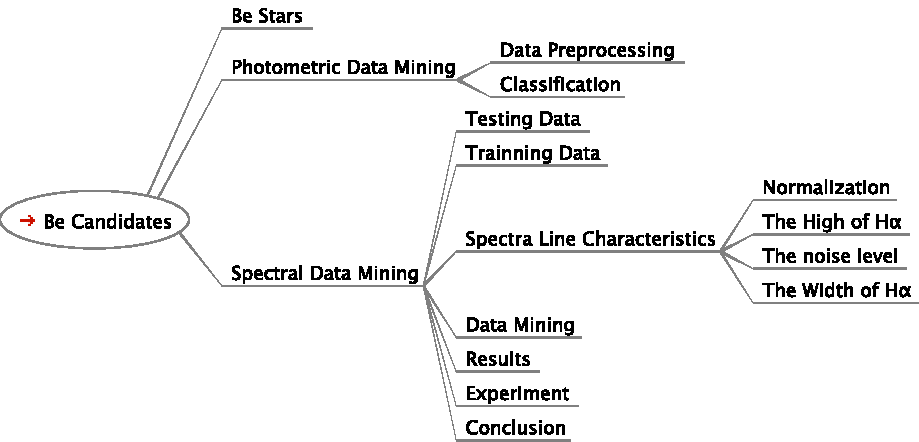
\includegraphics[scale = 1]{mapBeCandidates}
    \else
    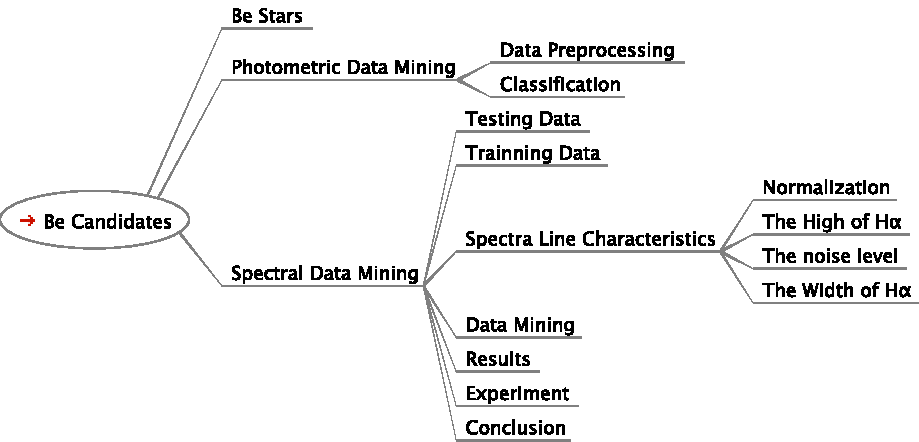
\includegraphics[bb = 92 86 545 742, height=6in]{mapBeCandidates} 
    \fi
    \caption{Chapter structure}
    \label{FigStructure}
  \end{center}
\end{figure}


\noindent Astronomical objects used in this work to demonstrate some
of the discussed technologies and methods were Be stars. The goal was
to develop a process of finding new candidates in the available
data. Several approaches were considered and two of them are discussed
in the rest of this text. The first one utilizes photometric
properties of Be stars, the second one their spectra characteristics.


\section{Be stars}
\label{sec:be}
The first example of Be star ($\gamma$ Cas) was reported by Padre Angelo
Secchi in his letter to the Astronomische Nachrichten in 1866.

Classical Be stars are non-supergiant B-type stars whose spectrum has
or had at some time, one or more Balmer lines in emission. The current
accepted explanation of this phenomena is circumstellar gaseous
component in the form of equatorial disk. The rapidly rotating central
star is important feature of these objects, which may be important
contributor of the circumstellar medium. It is estimated that about 20
percent of B stars are in fact Be stars. As the definition suggests,
the spectra of Be stars can vary with time. Related to the Be stars
are the shell stars: B stars with deep and narrow absorption lines in
their spectra, superimposed on the normal broad absorption lines of
hydrogen and helium which dominate their spectra. Stars can actually
change from B to Be to B-shell and back to B again. Finally, there are
variations on time scales of 0.3 to 2 days, which are due to
non-radial pulsation, or perhaps rotation. These variations, which
occur on or near the surface of the star, may be connected with the
formation of the disc around the star \citep{porter2003classical}.

The important characteristic used later in the work is the H$\alpha$
emission. The explanation of its origin is on following pictures.


    \begin{figure}[!htbp]
      \begin{center}
        \leavevmode
        \ifpdf
        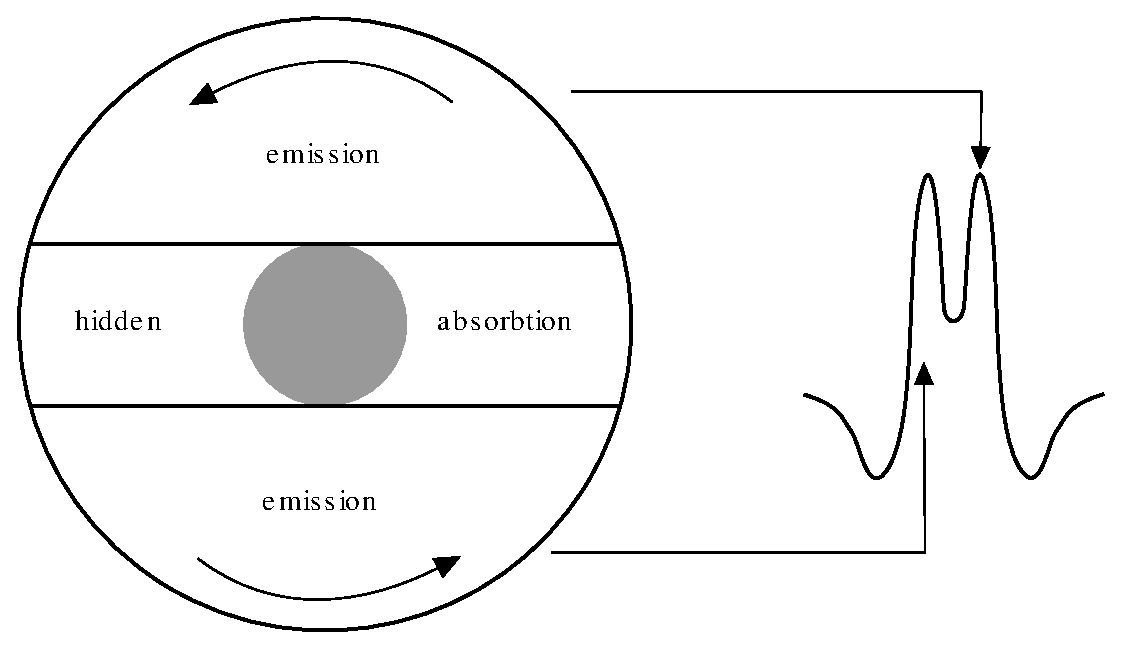
\includegraphics[scale =.6]{beStarLine}
        \else
        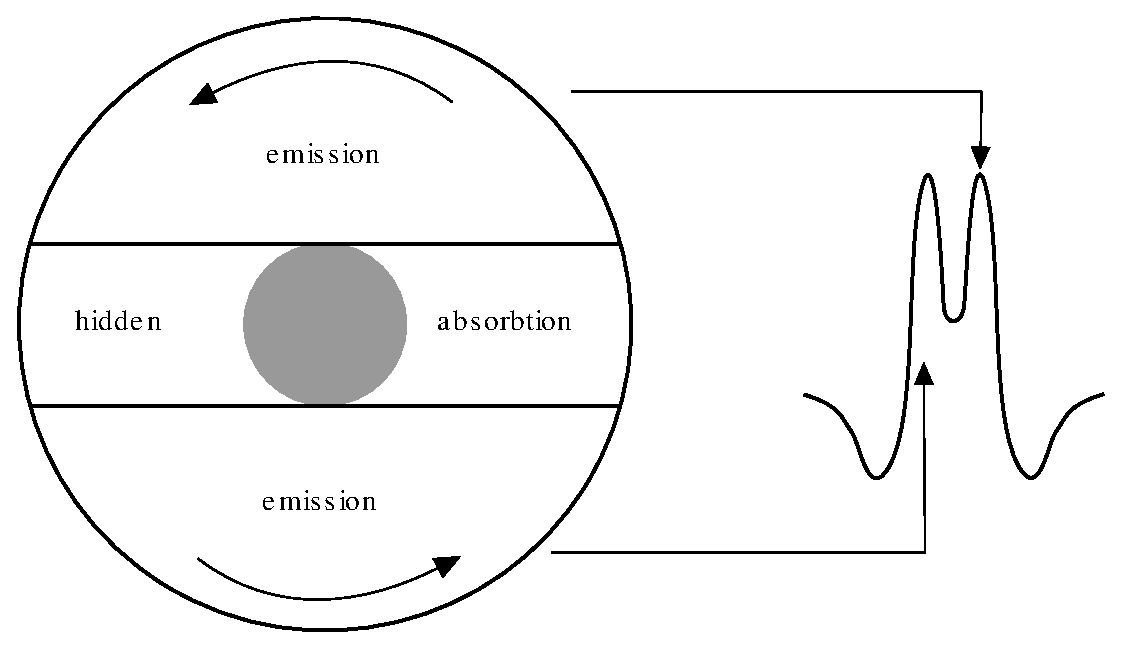
\includegraphics[bb = 92 86 545 742, height=6in]{beStarLine}
        \fi
        \caption{A model of a typical Be star. Emission lines coming
          from an equatorial disk is added to the photo-spheric
          absorption spectrum. Central B star emits UV (Lyman
          continuum) and ionizes the disk, which in turn re-emits at
          high wavelength such as visible domain
          \citep{hirata1984star}}
        \label{Figjhk_be_b}
      \end{center}
    \end{figure}


    \begin{figure}[!htbp]
      \begin{center}
        \leavevmode
        \ifpdf
        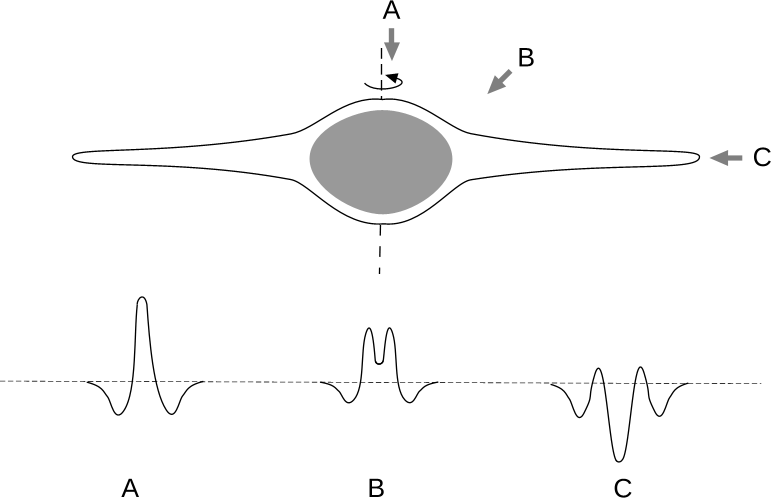
\includegraphics[scale =.6]{beStarLine2}
        \else
        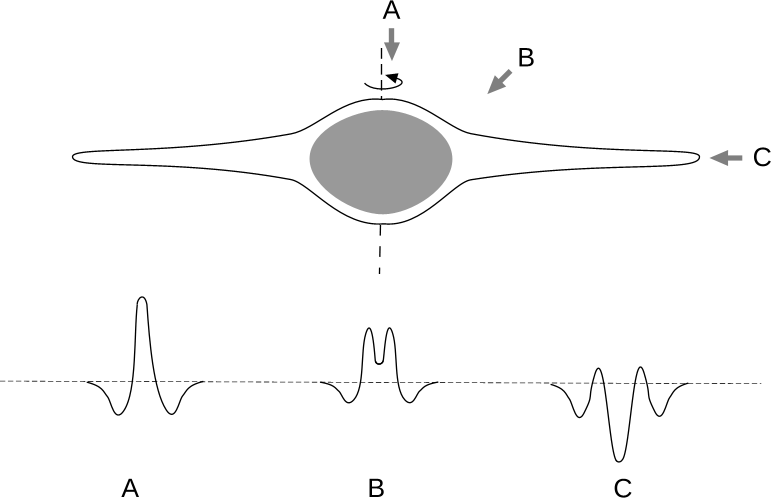
\includegraphics[bb = 92 86 545 742, height=6in]{beStarLine2}
        \fi
        \caption{Example of spectra of Be stars based on view angle
          \citep{slettebak1988stars}}
        \label{Figjhk_be_b}
      \end{center}
    \end{figure}
 
\clearpage

    There are still many open questions related to their rotation,
    evolutionary status, presence and origin of the magnetic fields,
    mass and angular momentum transfer and others, therefore the
    process for automatic discoveries of Be phenomena in the digitized
    surveys and obtaining new candidates could help to answer these
    questions.


\section{Photometric Data Mining}

% The question I have tried to answer in this chapter was: Is it
% possible to find Be stars candidates based on photometric properties
% only? To answer this question I needed training set of confirmed Be
% stars, set of non Be stars (spectral type B was considered) and some
% Data Mining algorithm to perform classification.

   \begin{figure}[!htbp]
      \begin{center}
        \leavevmode
        \ifpdf
        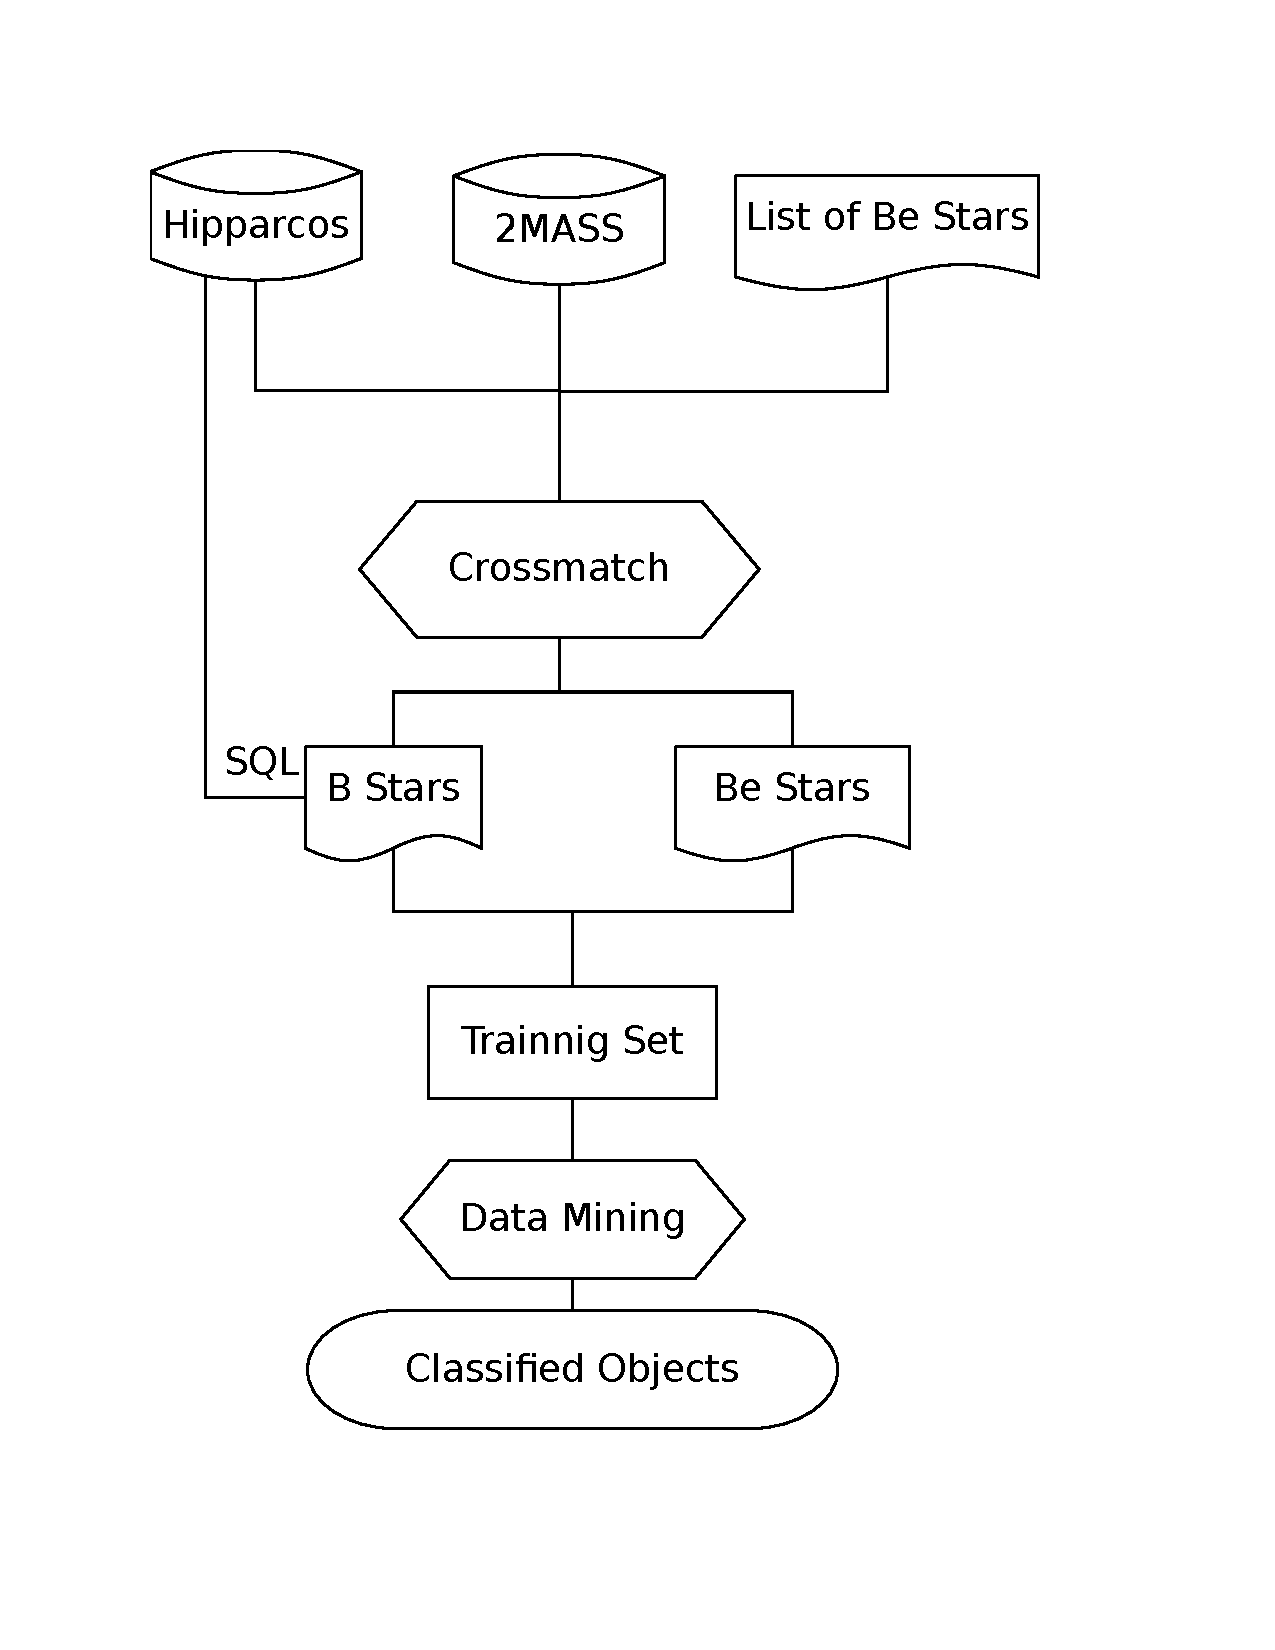
\includegraphics[scale =.5]{flowPhoto}
        \else
        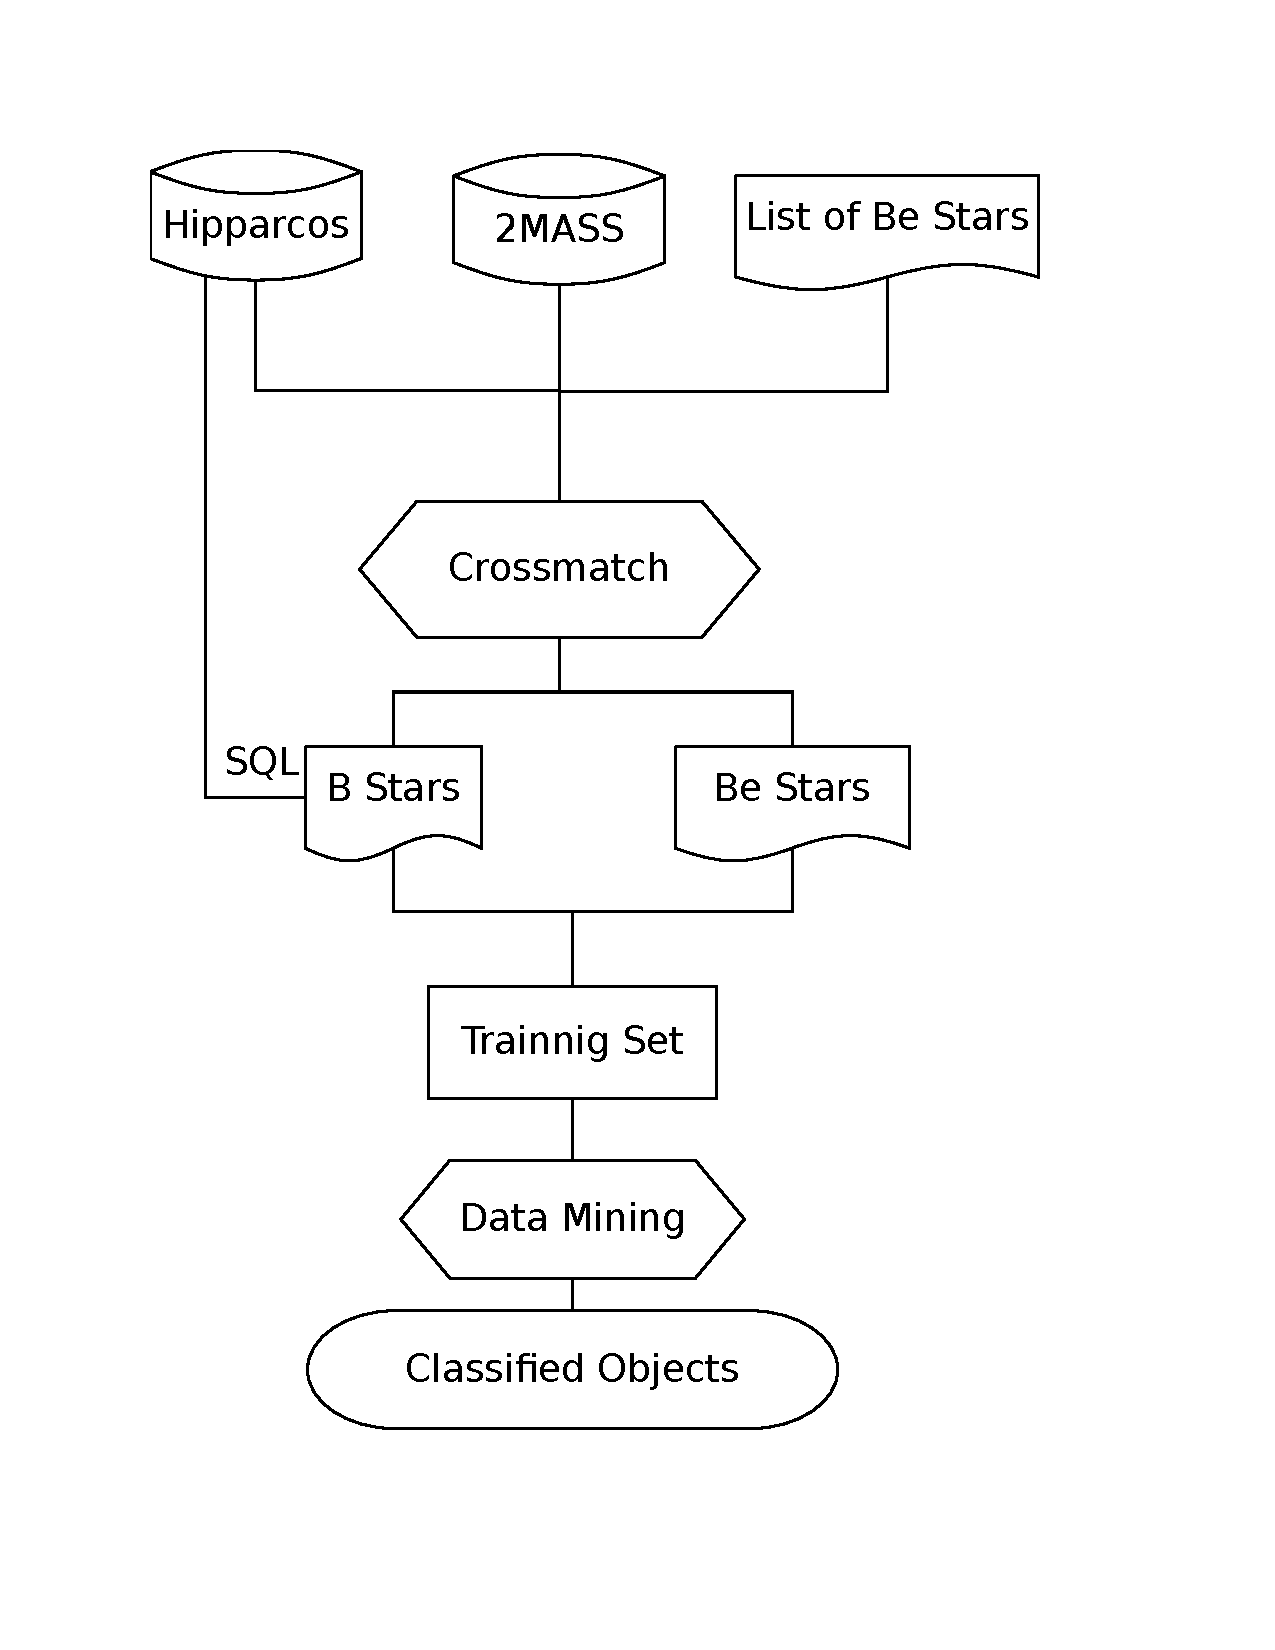
\includegraphics[bb = 92 86 545 742, height=6in]{flowPhoto}
        \fi
        \caption{A schematic diagram of the photometric Data Mining
          process. The lists of confirmed Be stars consisted of
          Hipparcos IDs, this was correlated with Hipparcos catalog to
          obtain right ascension and declination of the objects and
          subsequently cross-matched with 2MASS catalog to get
          photometric data. The second set of B stars was acquired in
          similar manner but using SQL the condition was set to get B
          type stars different from the list of Be stars}
        \label{FigFlowSpectra}
      \end{center}
    \end{figure}

 
%\clearpage



    The classification based on photometric properties is very
    attractive from several points of view. There are much more
    available photometric then spectral data and they are more
    accessible. Because they are easier to acquire the disproportion
    between photometric and spectral data will probably increase in
    the future as well. The distinction between Be and other types of
    stars also should be theoretically possible since the Be stars
    exhibit infrared excess correlated to the H$\alpha$ emission
    \citep{van1995halpha}.

Color indices were computed from 2MASS catalog which uses JHK
photometric system. The filters JHK are an important extension of the
Johnson system to near-infrared wavelengths.

\begin{table}[ht]
  \centering
  \small
     \begin{tabular}[ht]{l c}
     \toprule
     Filter & Effective wavelength [$\mu\textrm{m}$] \\
     \midrule
     J & $1.235 \pm 0.006$ \\
     H & $1.662 \pm 0.009$ \\
     $K_s$ & $2.159 \pm 0.011$ \\
     \bottomrule
   \end{tabular}
   \caption{JHK photometric system \citep{cohen2003spectral}}
  \label{tab:JHKFilter}
\end{table}



\subsection{Data preprocessing}

The process is depicted in figure \ref{FigFlowSpectra}. The list of
confirmed Be stars is from Astronomical Institute of the Academy of
Science in Ond\v{r}ejov. The list contains Hipparcos IDs
\citep{perryman1997hipparcos} of objects carefully checked in
scientific papers. Correlation with Hipparcos was done using
cross-matching function in STILTS application. The second part of the
training set (stars different then Be) were obtained using SQL query
against Hipparcos catalog. B stars were used as they are the most
similar. J,H,K colors were obtained from 2MASS
\citep{skrutskie2006two} using method of multi-cone search protocol of
Virtual Observatory.


%   I was provided with a
% list of confirmed Be stars (Hipparcos IDs) from Astronomical Institute
% of the Academy of Science in Ond\v{r}ejov. The list contained 625
% manually chosen objects (their Hipparcos IDs). These IDs were used to
% query Hipparcos catalog \citep{perryman1997hipparcos} to obtain their
% ICRS RA, DEC. Having these coordinates 2MASS \citep{skrutskie2006two}
% catalog was used to obtain J,H,K colors using method of multi-cone
% search in Virtual Observatory. The complementary part of training
% non-Be stars set was acquired from Hipparcos catalog using following
% SQL query:

\begin{lstlisting}
  Select * 
  From maincat as m, hipva1 as h 
  Where  (m.HIP=h.HIP )  
  And h.SpType Like 'B%'
\end{lstlisting}

The result was cross-correlated with 2MASS catalog to obtain the same
colors as for the confirmed Be stars. Color digram of this two sets is
in the figure \ref{Figjhk_be_b}

    \begin{figure}[!htbp]
      \begin{center}
        \leavevmode
        \ifpdf
        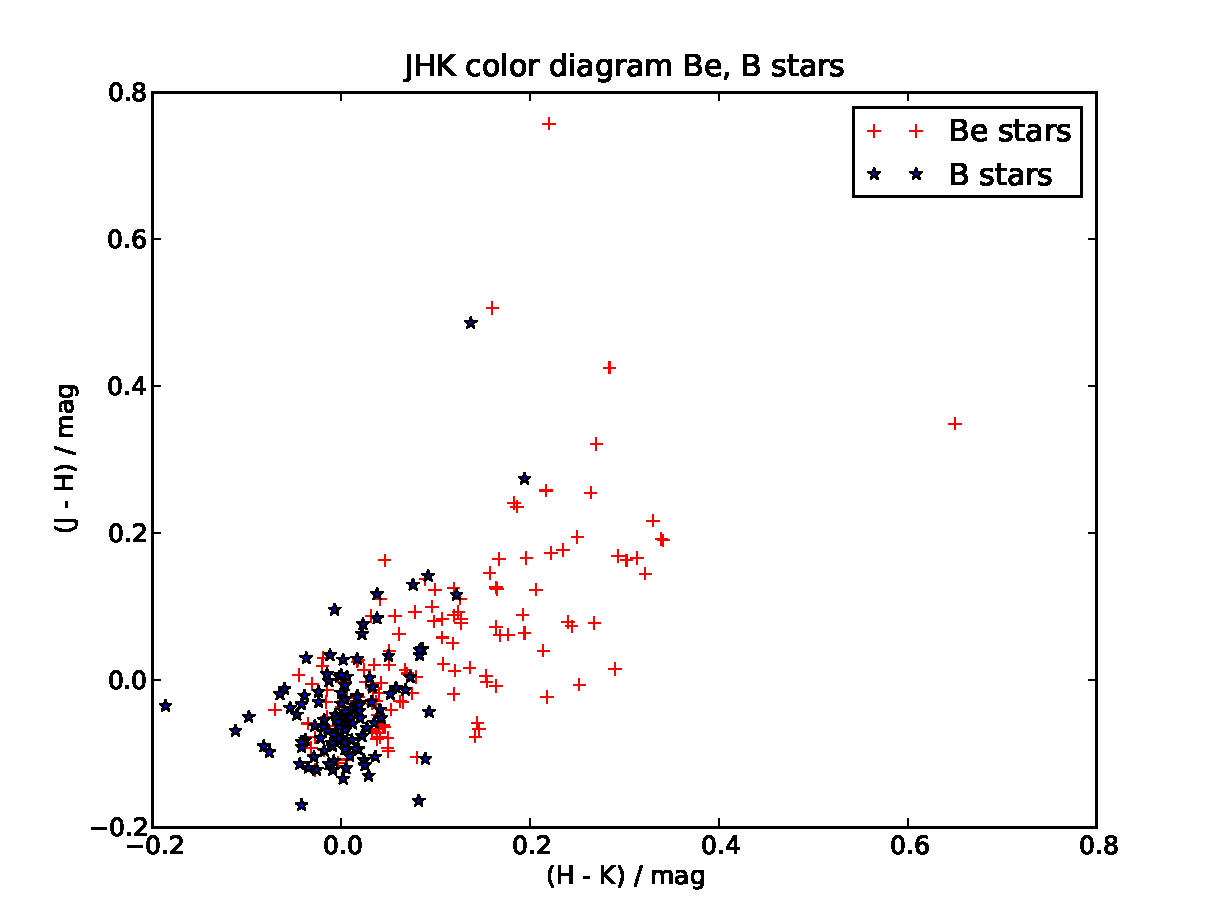
\includegraphics[scale =.6]{jhk_be_b}
        \else
        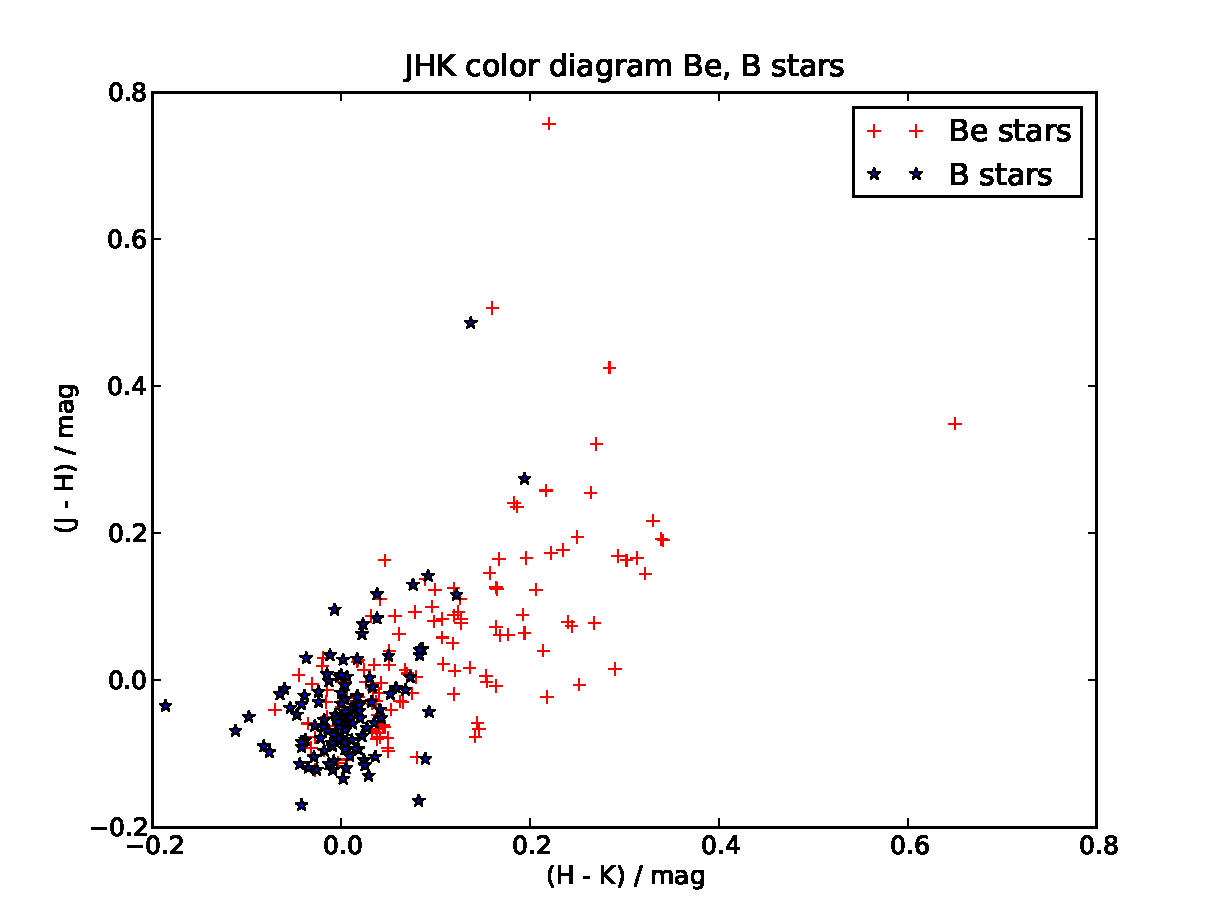
\includegraphics[bb = 92 86 545 742, height=6in]{jhk_be_b}
        \fi
        \caption{Color diagram of confirmed Be stars and B stars}
        \label{Figjhk_be_b}
      \end{center}
    \end{figure}

    The uncertainties were computed for each object using propagation
    of errors. Equation \ref{eq:error} shows example for $m_j - m_h$.
    The color digram with these error bars is depicted in the
    figure \ref{Figjhk_be_b_errors}. Although the uncertainties are
    significant certain trends are presented.

\begin{align}
\label{eq:error}
  \delta_{(m_j - m_h)} &= \sqrt{\left(\frac{\partial(m_j - m_h) }{\partial
        m_j}\right)^2\delta_{m_j}^2 + \left(\frac{\partial(m_j - m_h) }{\partial
        m_h}\right)^2\delta_{m_h}^2} \\
  \frac{\partial(m_j - m_h) }{\partial m_j } &= 1,\frac{\partial(m_j - m_h)
  }{\partial m_h } = -1 \\
  \delta_{(m_j - m_h)} &= \sqrt{\delta_{m_j}^2 + \delta_{m_h}^2}
\end{align}


    \begin{figure}[!htbp]
      \begin{center}
        \leavevmode
        \ifpdf
        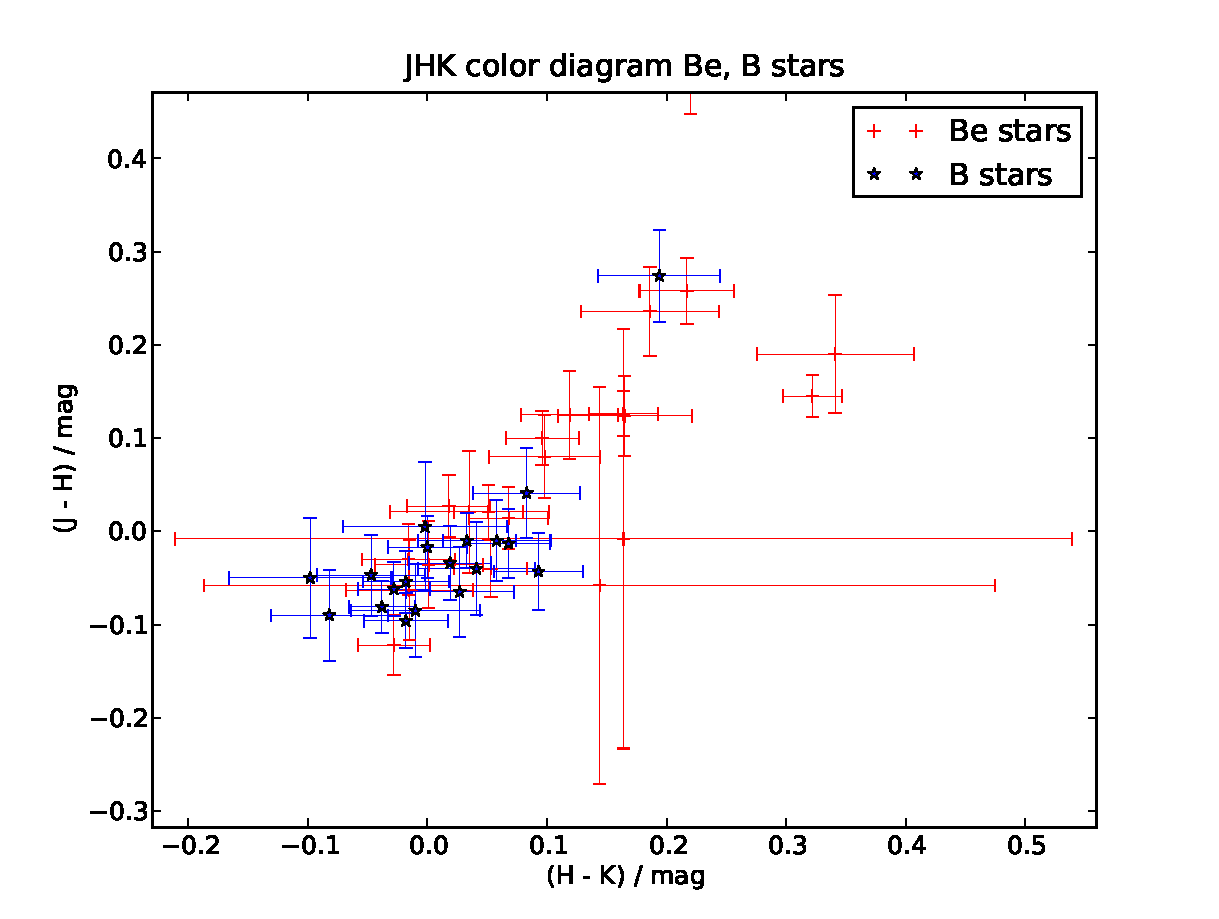
\includegraphics[scale =.6]{jhk_be_b_errors}
        \else
        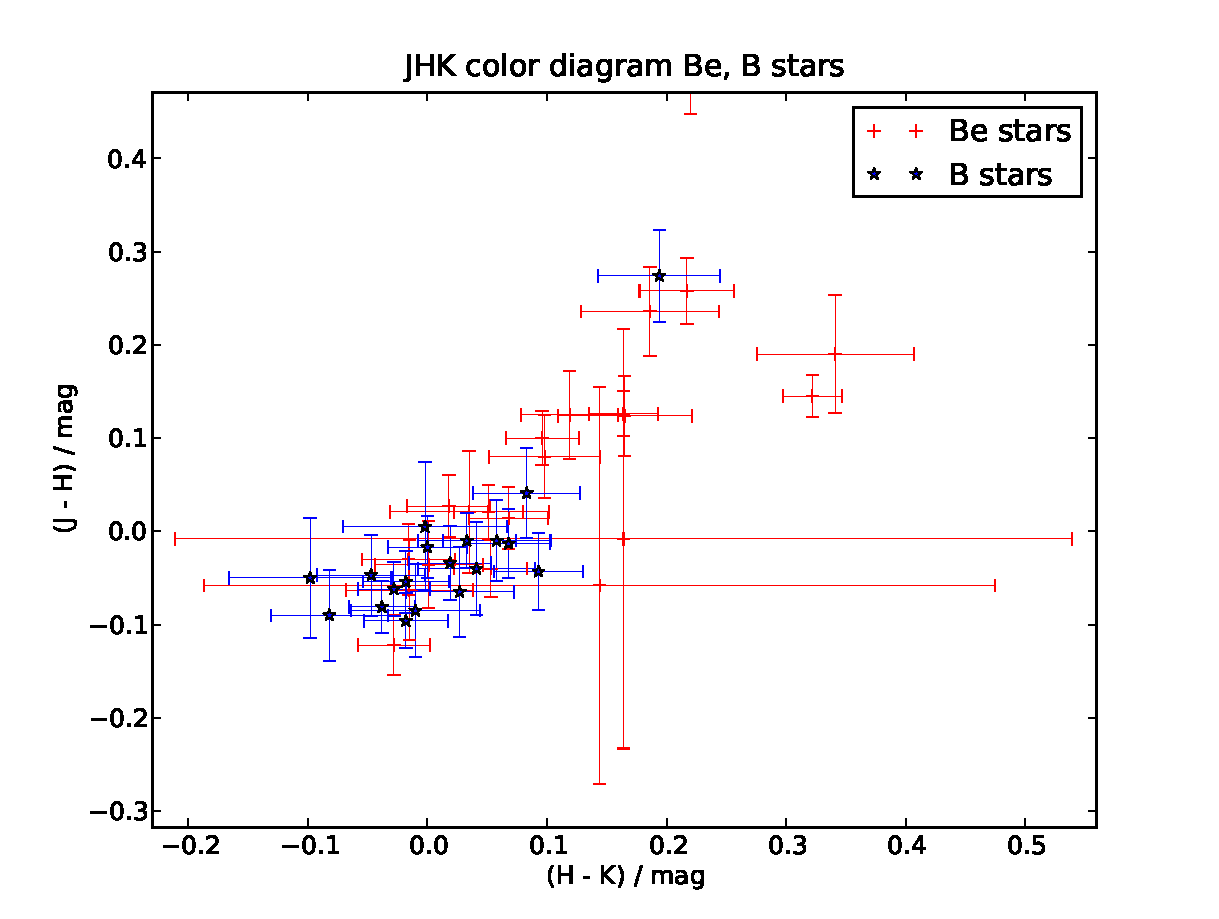
\includegraphics[bb = 92 86 545 742, height=6in]{jhk_be_b_errors}
        \fi
        \caption{Color diagram of confirmed Be stars, B stars with errors}
        \label{Figjhk_be_b_errors}
      \end{center}
    \end{figure}

%\clearpage


\subsection{Classification}
Data were transformed from original VOTable obtained from Virtual
Observatory tools to arff\footnote{Attribute-Relation File
  Format. Developed by the Machine Learning Project at the Department
  of Computer Science of The University of Waikato.}format used in
Weka Data Mining system. Algorithm C4.5 (J48) was used to perform
actual classification with following result:

\begin{lstlisting}
  Correctly Classified Instances         769               73.0989 %
  Incorrectly Classified Instances       283               26.9011 %
  Kappa statistic                          0.4496
  Mean absolute error                      0.3843
  Root mean squared error                  0.4383
  Relative absolute error                 79.4985 %
  Root relative squared error             89.1648 %
  Total Number of Instances             1052
\end{lstlisting}

As seen on the first row 73 \% from  1052 objects were classified
correctly. More details can be obtained from confusion matrix below.

\begin{lstlisting}
  B   Be   <-- classified as
 304 126 |   B
 157 465 |   Be
\end{lstlisting}

304 of B and 456 of Be stars were classified correctly but 126 of B
and 157 of Be stars were classified incorrectly. In virtue of these
results one should be sceptical if the distinction based only on
photometric properties is significant enough to find relevant new
candidates of Be stars. On the other side, as mentioned in
\ref{sec:be}, about 20 percent of B stars are estimated to be Be
stars. For this and other reasons more sophisticated (and much more
complicated) approach using spectra analysis was tested.

\section{Spectral Data Mining}
\label{sec:spectral}

   \begin{figure}[!htbp]
      \begin{center}
        \leavevmode
        \ifpdf
        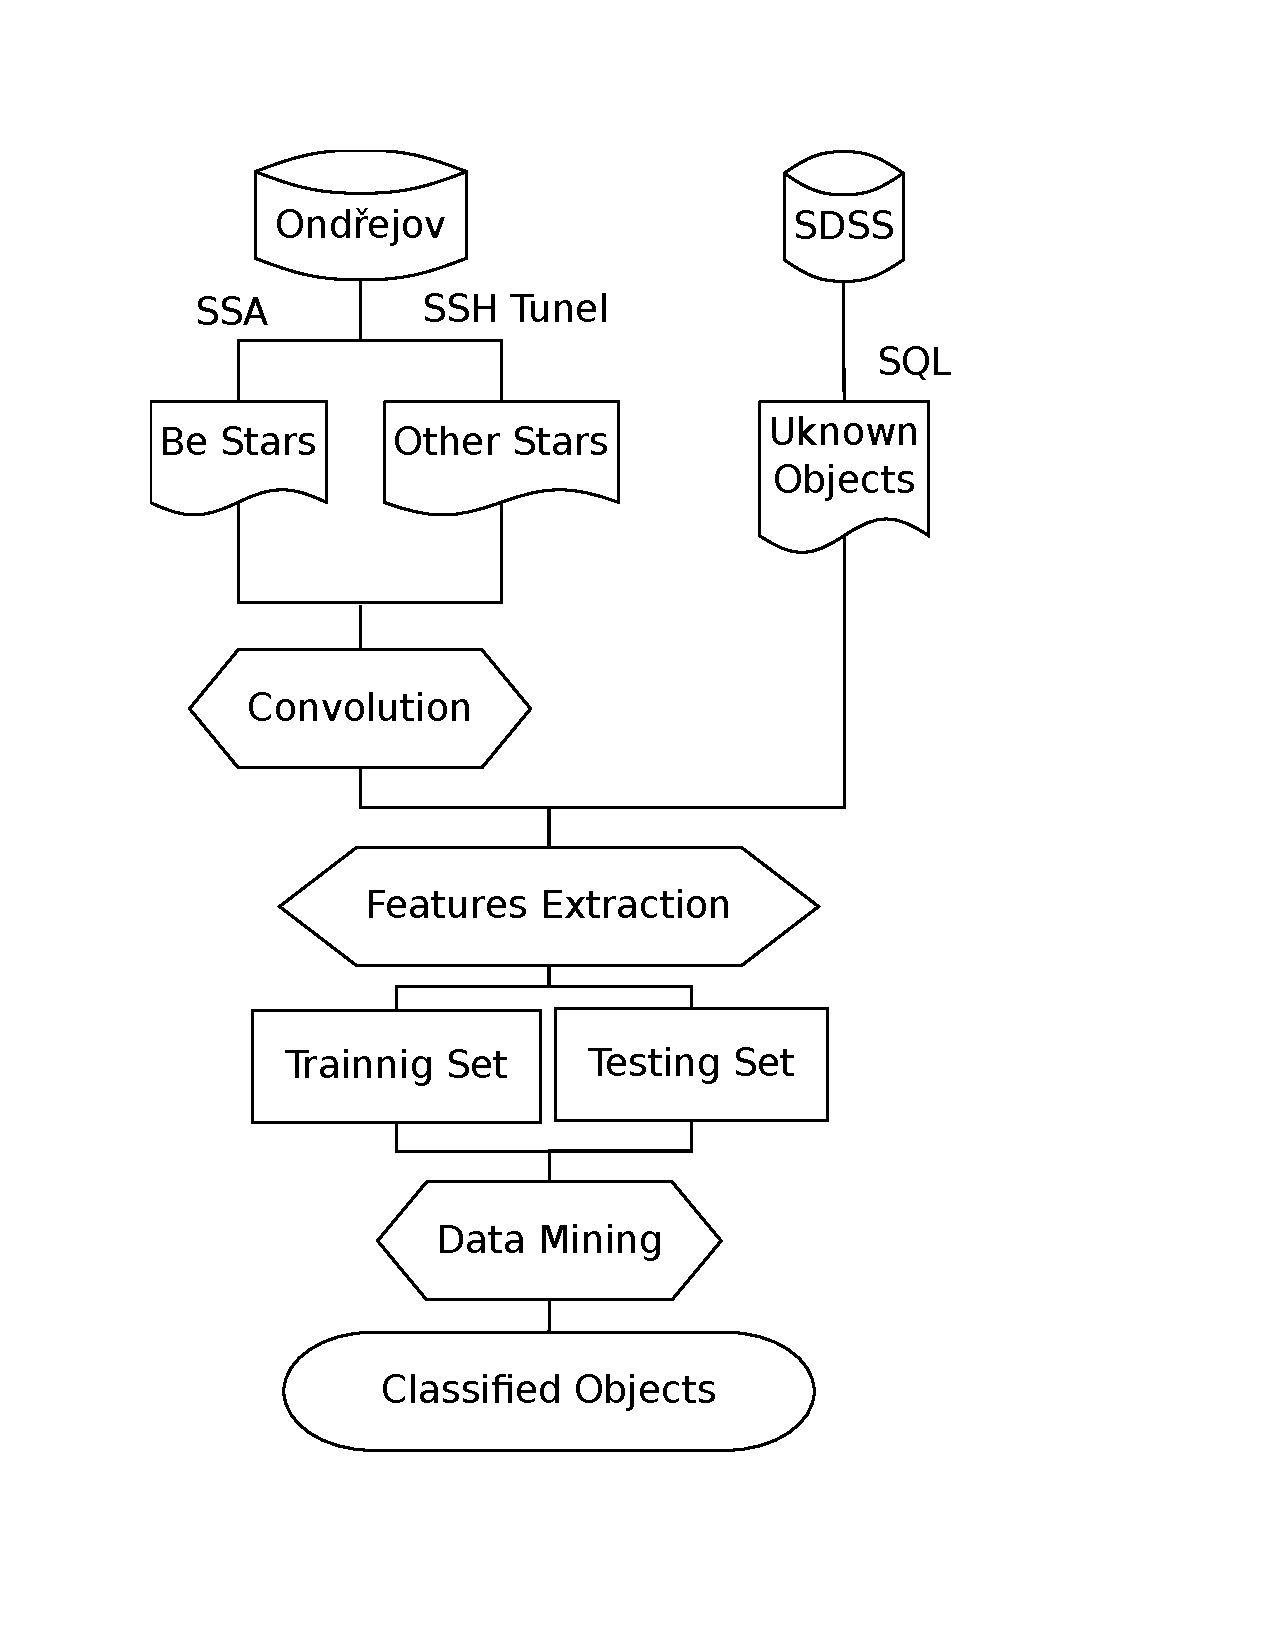
\includegraphics[scale =.5]{flowSpectra}
        \else
        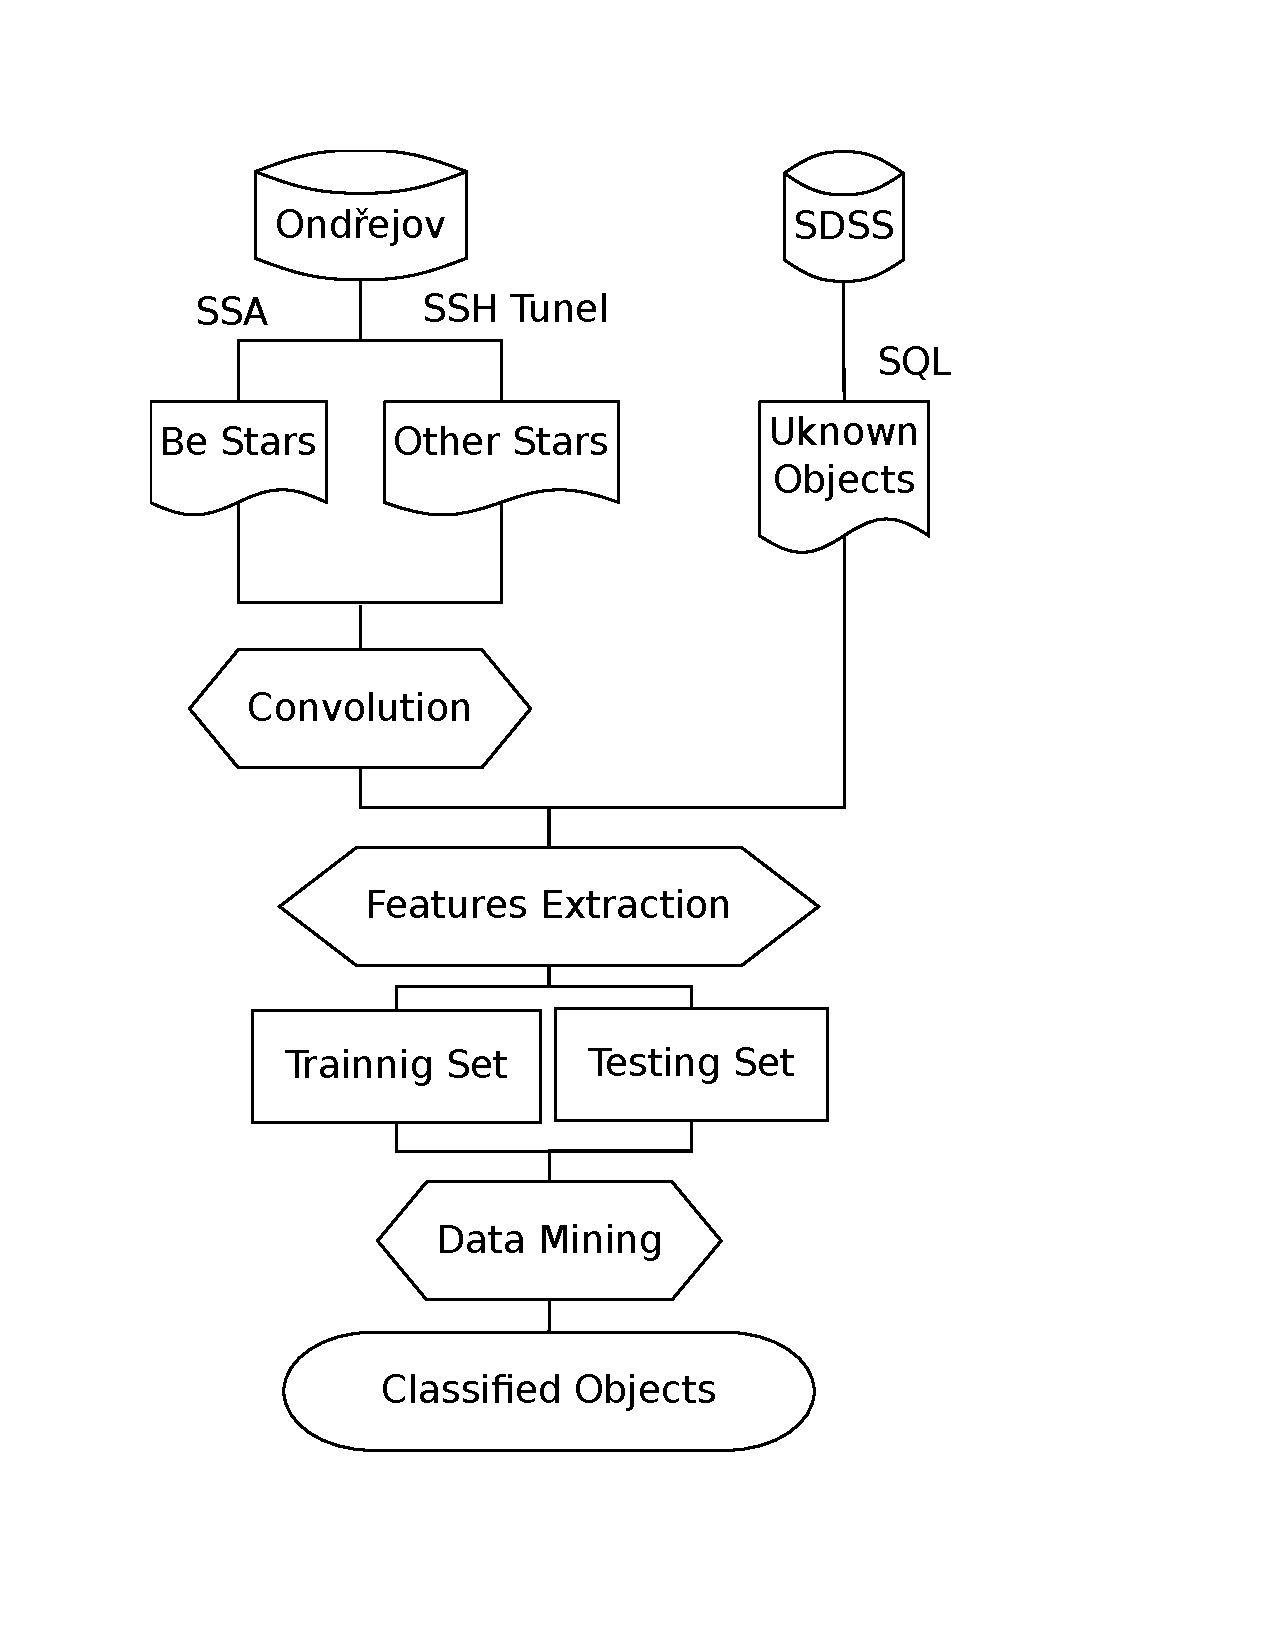
\includegraphics[bb = 92 86 545 742, height=6in]{flowSpectra}
        \fi
        \caption{A schematic diagram of the spectral data mining
          process. Using SSA protocol the spectra from Ond\v{r}ejov server
          were acquired based on the list from photometric study. %SSH
          %Tunneling was necessary since Ond\v{r}ejov spectra are top
          %secret and therefore not available to the public.
          Convolution with SDSS instrumental profile had to be
          performed to ensure compatibility with SDSS. Afterwards the
          desired features were extracted automatically from the
          spectra after the continuum normalization and H$\alpha$ line
          was fitted by appropriate function. The same was done for
          spectra from SDSS except the convolution process}
        \label{FigFlowSpectra}
      \end{center}
    \end{figure}

 
%\clearpage

    Spectra provide much wider scientific information over photometric
    properties. Spectral lines exhibit many distinguished features and
    astronomers have long tradition in analysing their properties. On
    the other hand it is much more complicated to handle them because of
    different characteristics (resolution, calibration, wavelength
    range, etc.). This is especially true for massive automated
    processing.

\subsection{Testing Data}
As testing sample the spectra from project SEGUE of SDSS were
selected. This contains 178315 spectra in DR7. Following SQL query was
used to generate the list of URL links for individual FITS
files. These files were then downloaded to local sever using
\textrm{wget} command.

\begin{lstlisting}
SELECT  objid,dbo.fGetUrlFitsSpectrum(s.specObjID)                                                           
FROM SpecPhotoAll s, platex p                                                                         
WHERE s.specObjID is not null                                                                         
AND s.plateid = p.plateid                                                                             
AND p.programname LIKE 'segue%'                                                                       
AND specClass = 1
\end{lstlisting}

\subsection{Training Data}
The spectra obtained with coud\`e spectrograph of Ond\v{r}ejov
Observatory 2m telescope were used as a training sample. Files were
downloaded using SSA protocol. The SSA server is not publicly
accessible outside of the local network of Ond\v{r}ejov observatory.
That is why the SSH tunneling of HTTP protocol was used. Two scripts
for this process were created. First to construct the list of SSA
compliant addresses, the second to analyse acquired response in
VOTable format. Then the spectra were downloaded using \emph{wget}
command.

% The function for constructing the links
%     based on list of the RA, DEC which were obtained from Hipparcos
%     catalog using the specification of IDs from Ondřejov's index.

\begin{lstlisting}
def createQuery(data):
    """ From raw data construct ra, dec """
    """ Convert to degrees """
    for line in data:
        ra = ac.AngularCoordinate(line[0:10]).degrees # convert ra to degrees
        dec = ac.AngularCoordinate(line[-13:-1]).degrees # convert dec to degrees
        ra = line[0]
        dec = line[1]
        ssaTemp = 'http://tvoserver/coude/coude.cgi?c=ssac&n=coude_ssa&REQUEST=queryData&POS=<ra>,<dec>&SIZE=1'
        ssaTemp = ssaTemp.replace('<ra>',"%0.3f" % ra)
        ssaTemp = ssaTemp.replace('<dec>',"%0.3f" % dec)
        ssa.append(ssaTemp)
    return ssa
\end{lstlisting}

The script generates the following output. The same process was used
later for obtaining the sample of non-Be stars.

\begin{lstlisting}
http://tvoserver/coude/..._ssa&REQUEST=queryData&POS=83.113,-65.582&SIZE=60
http://tvoserver/coude/..._ssa&REQUEST=queryData&POS=162.537,148.333&SIZE=60
http://tvoserver/coude/..._ssa&REQUEST=queryData&POS=19.907,-73.502&SIZE=60
\end{lstlisting}


\subsubsection{Degradation of Spectral Resolution}
Because spectra from Ond\v{r}ejov Observatory have higher spectral
resolution than SDSS, the degradation of spectral resolution was
applied on them. Wavelength for spectra from Ond\v{r}ejov Observatory
is computed using formula:

\begin{equation}
  \label{eq:computeWave1}
  \lambda = \lambda_0 + x\Delta\lambda_{OND} 
\end{equation}

\noindent and for SDSS spectra by equation:

\begin{equation}
  \label{eq:computeWave2}
  \lambda = 10^{\lambda_0 + x\Delta\lambda_{SDSS}},
\end{equation}

where $\lambda_0$ is value of parameter CRVAL1 and $\Delta\lambda$ of
CD1\_1. Obtaining them from FITS file is easy using
\textrm{PyFITS}\footnote{PyFITS is a product of the Space Telescope
  Science Institute, which is operated by AURA for NASA.}  module:

\begin{lstlisting}
  In [1]  import pyfits as pf
  In [2]: hdu = pf.open('sdss_test.fit')
  In [3]: hdu[0].header['CD1_1']
  Out[3]: 0.0001 # SDSS spectrum 
  Out[3]: 0.2567 # Ondrejov spectrum
\end{lstlisting}


\noindent From equations \ref{eq:computeWave1} and
\ref{eq:computeWave2} the ratio of spectral resolutions was computed:

\begin{equation}
  \label{eq:ratio}
  \frac{\Delta\lambda_{SDSS}}{\Delta\lambda_{OND}} \doteq  3.87
\end{equation}

\noindent Based on this computation 4 pixels of Ond\v{r}ejov spectra
were binned into one to conserve the number of pixels in extracted
spectral range. This is the critical part of the binning program:

\begin{lstlisting}
 def convolution(f, g):
    """ Convolve two functions"""
    fg = np.convolve(g,f,'same')
    return fg
 def reduce(x,y,bin):
    """ Reduce bin pixel into 1"""
    size = x.size/bin
    l = 0
    xx = x[:x.size-1:bin]
    yy = list()
    for i in range(0,size):
        s = 0
        for j in range(0,bin):
            s = s + y[l]
            l+=1
        yy.append(s/bin)
    return xx, yy
\end{lstlisting}

Prior to binning pixels the convolution with function representing the
instrumental profile of SDSS spectrograph was performed. As its first
order approximation the Gaussian function with $\sigma = 4$ pixels was
used:


\begin{equation}
  \label{eq:gauss}
  f(x) =  \mathrm{e}^{-\lambda^2/2\sigma^2}
\end{equation}

 Convolution is defined:

\begin{equation}
  \label{eq:convolution}
  (f * g )(\lambda) \stackrel{\mathrm{def}}{=}\ \int_{-\infty}^{\infty} f(\tau)\, g(\lambda - \tau)\, d\tau
\end{equation}
 
Here it was used in it's discrete form:

\begin{equation}
  \label{eq:discreteConvolution}
  (f * g)[n]\ \stackrel{\mathrm{def}}{=}\ \sum_{m=-\infty}^{\infty} f[m]\, g[n - m]
\end{equation}


The figure \ref{FigReduction} shows the result.

    \begin{figure}[!htbp]
      \begin{center}
        \leavevmode
        \ifpdf
        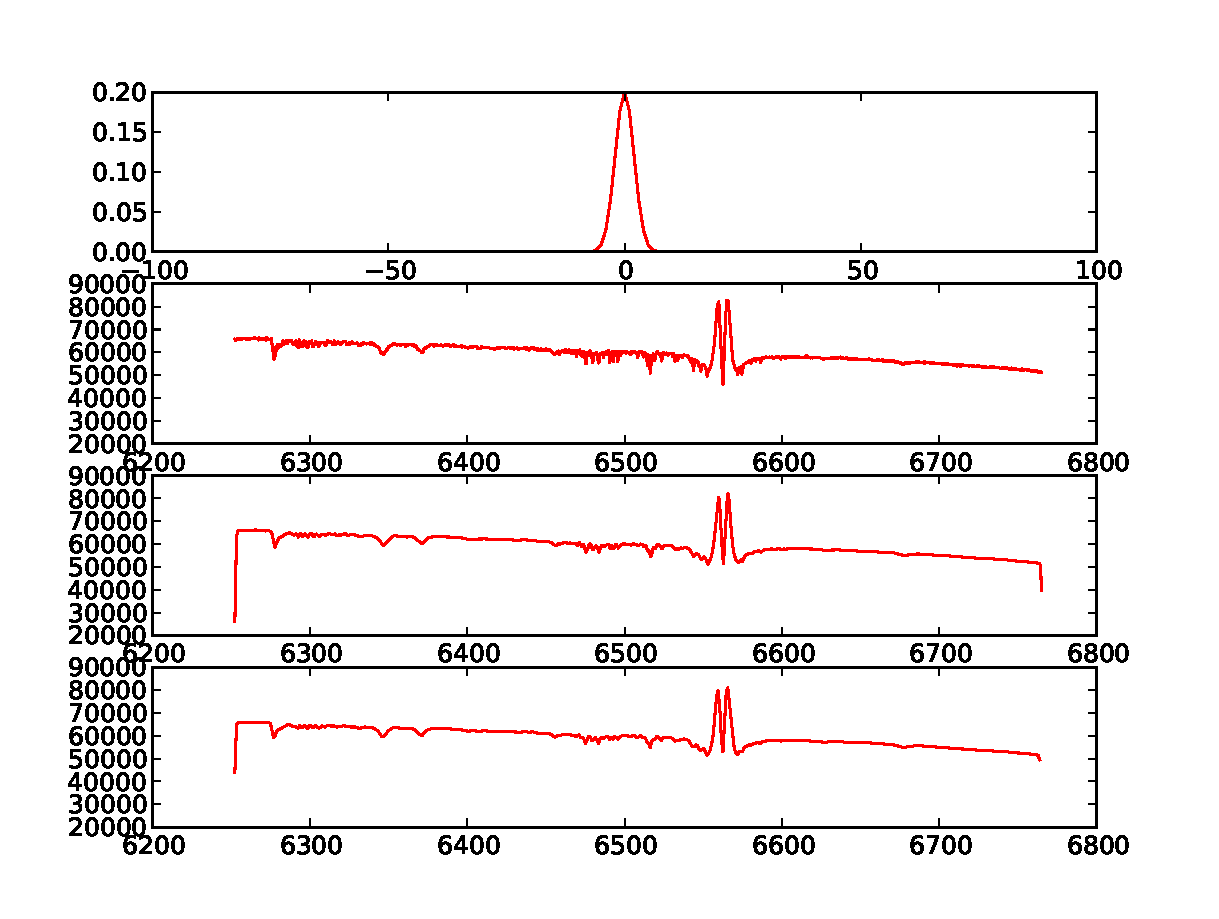
\includegraphics[scale =.8]{convolution}
        \else
        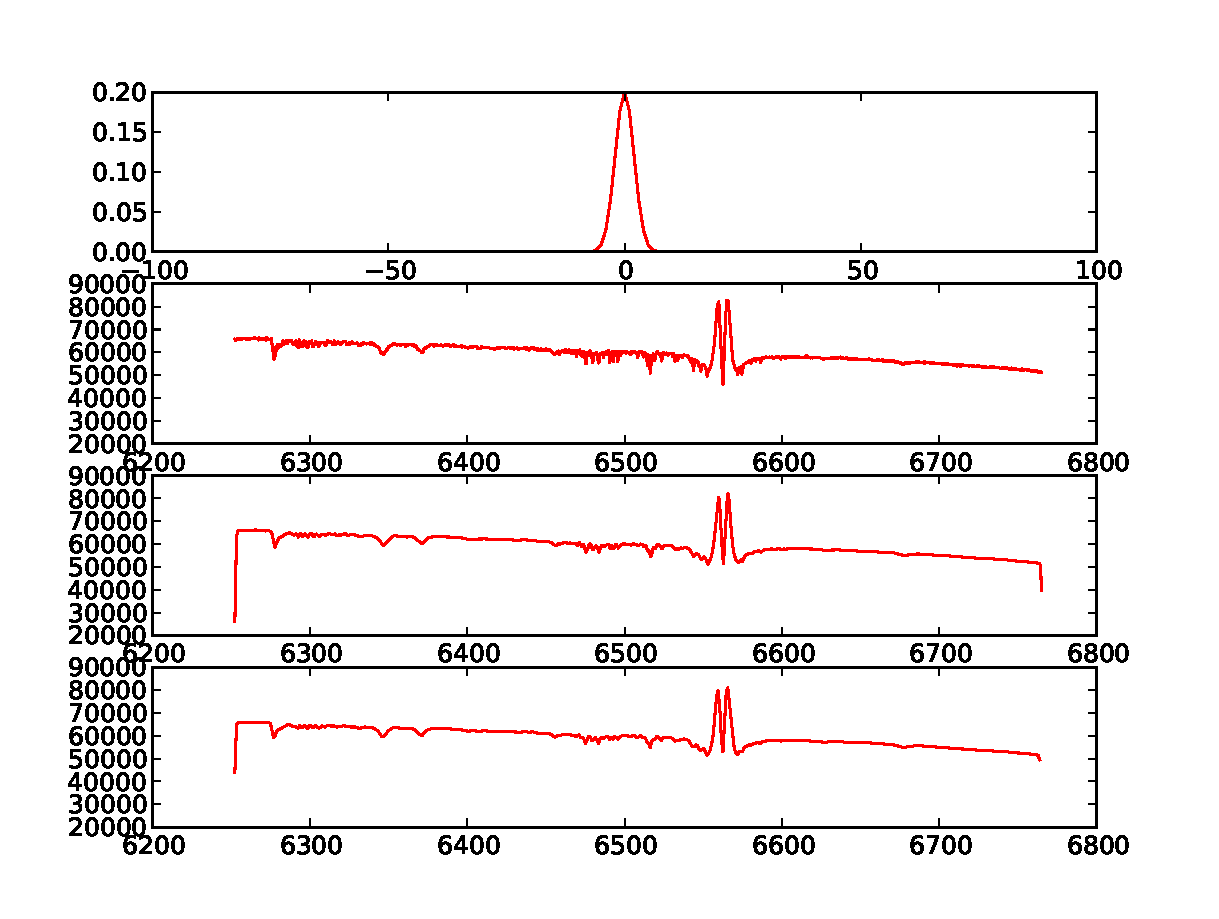
\includegraphics[bb = 92 86 545 742, height=6in]{convolution}
        \fi
        \caption{Reduction of spectral resolution of Ond\v{r}ejov
          spectra of the Be star 4 Her. The top figure shows Gaussian
          function used for convolution with the spectrum, followed by
          the original spectrum then there is a spectrum after
          convolution with the Gaussian profile. The last is the final
          spectrum after binning}
        \label{FigReduction}
      \end{center}
    \end{figure}

%\clearpage




\subsection{Spectral Lines Characteristics}
As parameters for data mining process characteristic values of
H$\alpha$ line were extracted from the spectra. Many possible
characteristics from different fitting functions through wavelet
coefficients to eigenvalues were discussed with experts. Three
parameters were finally selected. The height and the width of the
H$\alpha$ emission line and median absolute deviation as a
characterization of the noise level in the spectrum.


\subsubsection{Continuum normalization}
Spectra from SDSS are absolute flux calibrated, while the Ond\v{r}ejov
spectra state intensity only in ADUs. To be able to compare the size
and shapes of spectral line profiles the so called rectification of
spectra was performed. The spectra were divided by the linear function
roughly representing its (pseudo)continuum. This process ensures the
compatibility when comparing different spectra. Function polyfit from
numpy package was used to perform the fit. The solution minimizes the
squared error. To ensure the compatibility for data mining process
only the spectral range covered by Ond\v{r}ejov spectra
($6300-6800\AA$) was considered in SDSS spectra.


\begin{align}
  \frac{\partial}{\partial q_j} \sum_{i = 1}^n{[y_i -
    \operatorname{f}(q_j, x_i) ]^2} = 0,\hspace{2cm} j = 0,1
\end{align}

where 

\begin{align}
\operatorname{f}(x) = q_1x + q_0  
\end{align}


\subsubsection{The height of the H$\alpha$ line}
The maximum value in the region of $50\,\textrm{\AA}$ around H$\alpha$
above the linear fit was extracted from the spectrum.

\begin{lstlisting}
def getMax(x,y,line,range):
    """ Return maximum value of range in the spectrum"""
    xrange = x[(x < line + range) & (x > line - range)]
    yrange = y[(x < line + range) & (x > line - range)] - 1
    maximum = yrange.max()
    minimum = yrange.min()
    if abs(maximum)  > abs(minimum):
        extrem =  maximum 
    else:
        extrem = minimum 
    return xrange, extrem, sgn
\end{lstlisting}

\subsubsection{The noise level of the spectrum}
The noise in the spectrum contributes to the characteristics of the
spectral lines. As an estimator of the noise level the median
absolute deviation was used. It is defined as:

\begin{align}
  \operatorname{mad} = \operatorname{median}_{i}\left(\ \left| X_{i} -
      \operatorname{median}_{j} (X_{j}) \right|\ \right)
\end{align}

\subsubsection{The width of the H$\alpha$ line}
The Gaussian function:

\begin{align}
  \label{eq:gauss2}
  f(x) =  1 + e^{- { \frac{(x-x_0)^2 }{ S^2} } }
\end{align}

was fitted to the profile of H$\alpha$ spectral line. First the robust
estimators \citep{launer1979robustness} were computed and used as
input parameters for leastsq\footnote{"leastsqi"s a wrapper around
  MINPACK’s lmdif and lmder algorithms.} method from scipy.opt module,
which minimize the sum of squares.

\begin{align}
  x_0 & = \frac{\operatorname{median}(w_jx_j)}{\sum{w_i}}, \\
  S & = \frac{\operatorname{mad}(x_i - x_0)}{\sum{w_i}}.
\end{align}



Part of the script implementing fitting the Gaussian function

\begin{lstlisting}
x0 = np.median(sum(w*x))/sum(w)
S = sum(w*mad((x - x0)))/sum(w)
params = np.array([1, maximum, x0, S], dtype=float)
fit, flag = opt.leastsq(residuals, params, args=(yrange, xrange))
gauss = model(xrange, fit) + 1

def model(t, coeffs):
    return coeffs[0] + coeffs[1] * np.exp( - ((t-coeffs[2])/coeffs[3])**2 )
def residuals(coeffs, y, t):
    return y - model(t, coeffs)
\end{lstlisting}

Final results are in the figure \ref{FigSpecChar1} and
\ref{FigSpecChar2}. The script was adjusted to work with SDSS and
Ond\v{r}ejov spectra. The whole procedure was performed on all of the
cca 200 thousand SDSS spectra and almost 200 Ond\v{r}ejov spectra
resulting in the ASCII files with the characteristic values used later
in data mining process. The training set contains 173 confirmed Be
stars.

   \begin{figure}[!htbp]
      \begin{center}
        \leavevmode
        \ifpdf
        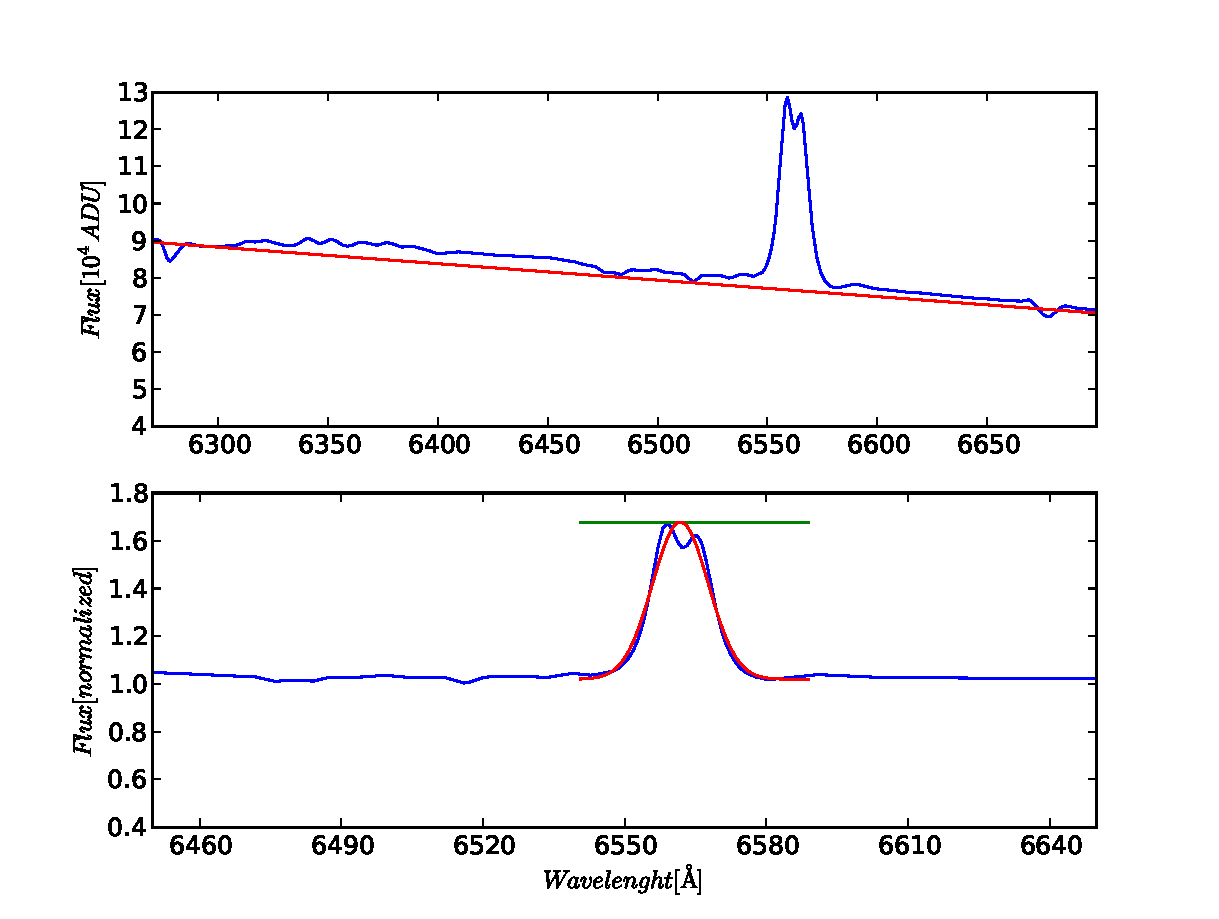
\includegraphics[scale =.8]{figSpecCharCyg60}
        \else
        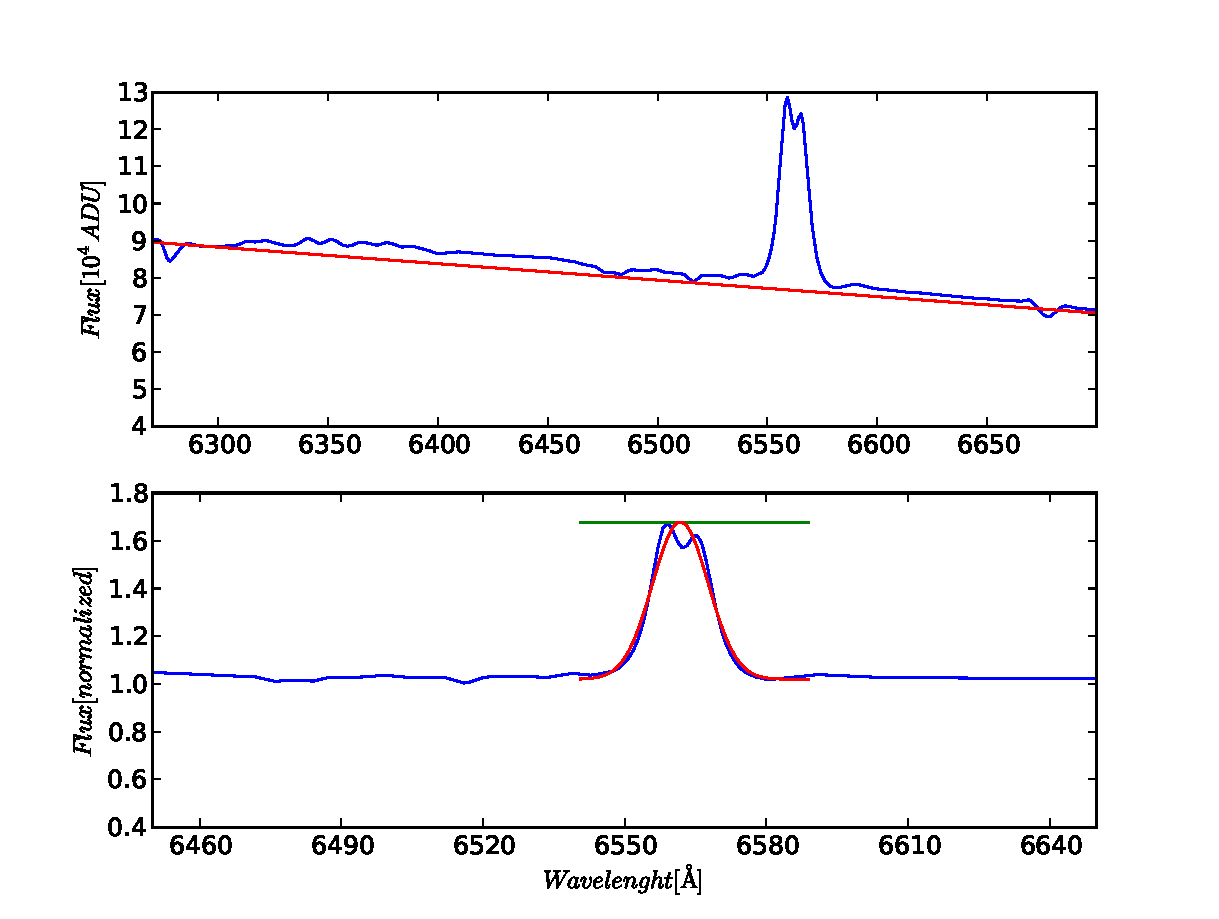
\includegraphics[bb = 92 86 545 742, height=6in]{figSpecCharCyg60}
        \fi
        \caption{Normalized spectrum of Be star 60 Cyg. The top figure
          depicts the continuum fit. The bottom figure shows the
          region (width of the green line) used for extraction. The
          position of the line corresponds to the maximum value in the
          region of $50\,\textrm{\AA}$. The Gaussian fit is in
          red. Although the fit is almost perfect, this approach fails
          to get characteristic double peak of the emission line }
        \label{FigSpecChar1}
      \end{center}
    \end{figure}

   \begin{figure}[!htbp]
      \begin{center}
        \leavevmode
        \ifpdf
        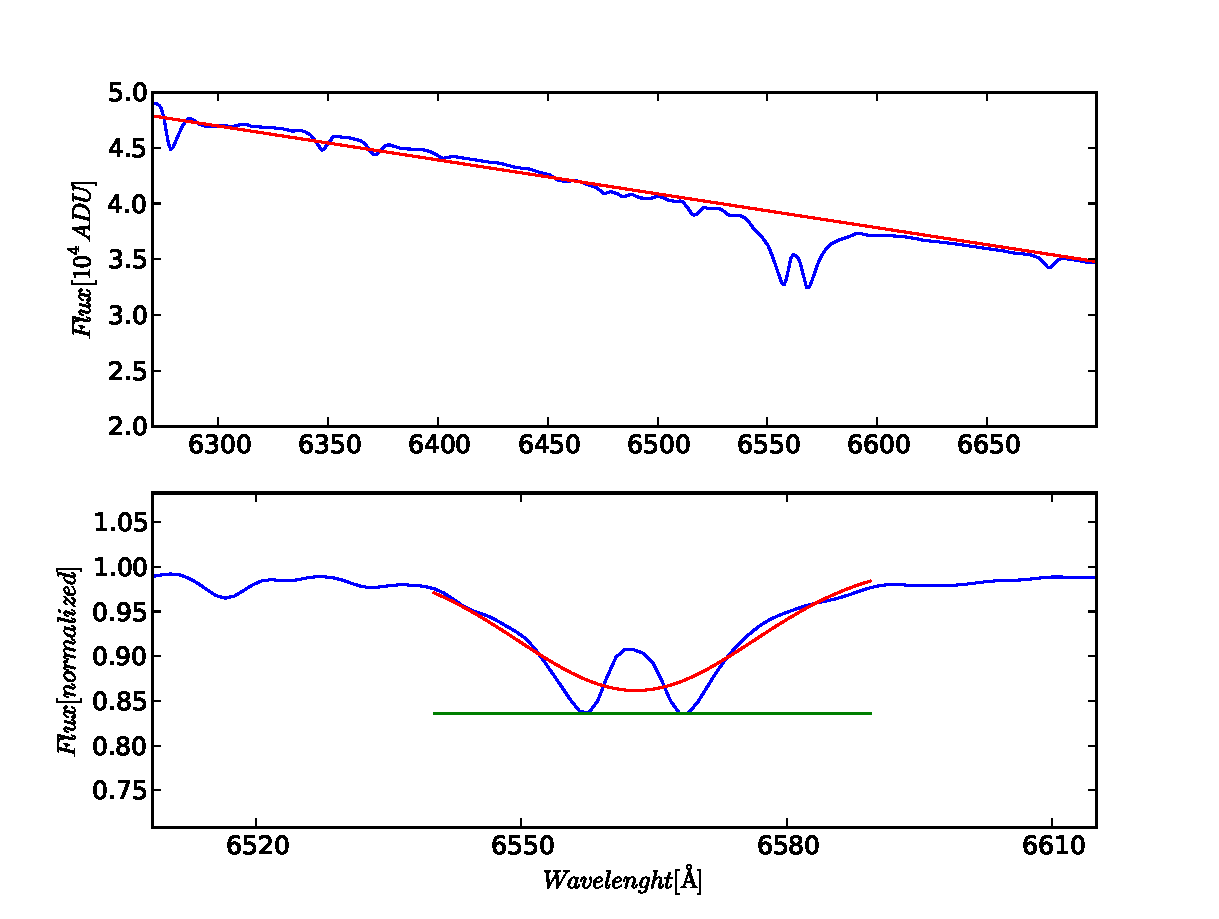
\includegraphics[scale =.8]{figSpecChar17tau}
        \else
        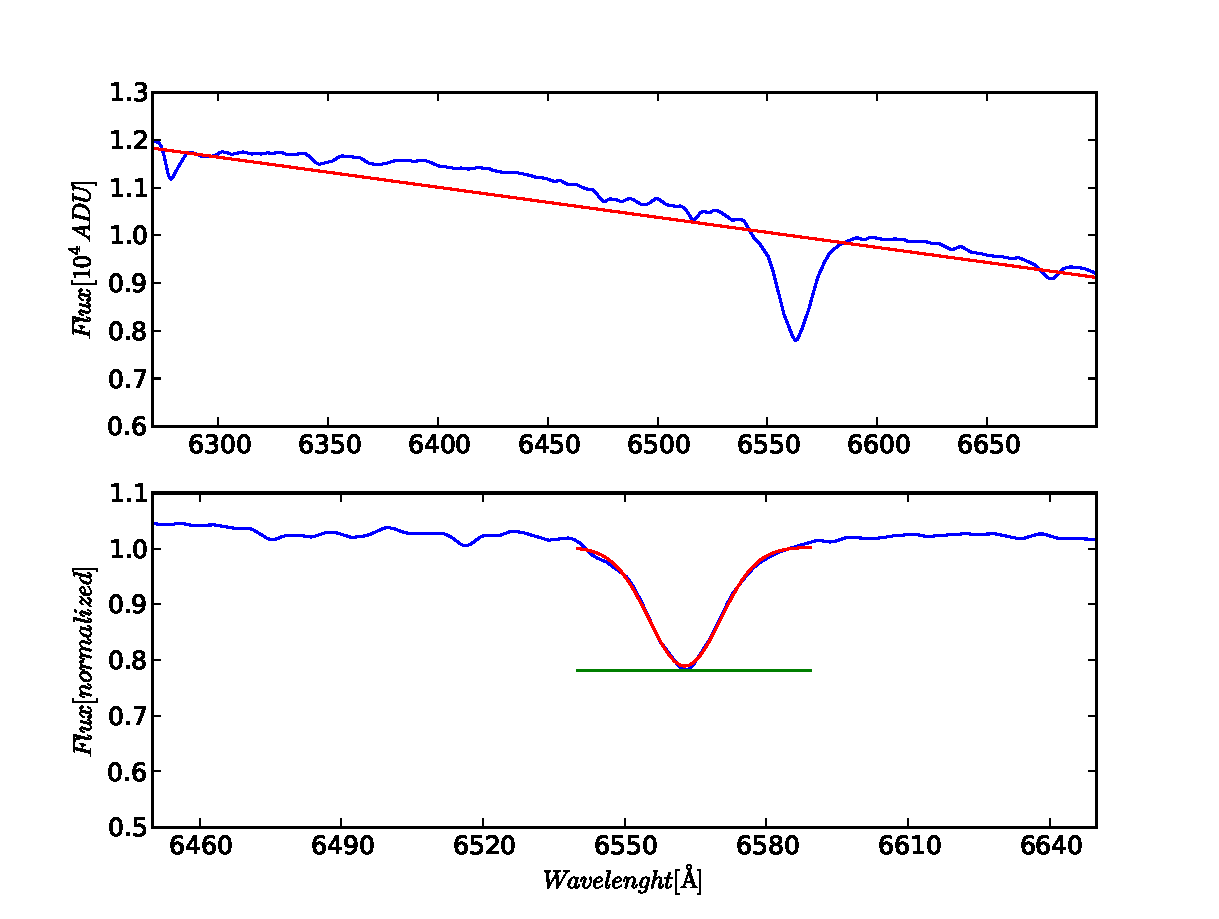
\includegraphics[bb = 92 86 545 742, height=6in]{figSpecCharhd216057}
        \fi
        \caption{Normalized spectrum of Be star 17 Tau. The top figure
          depicts the continuum fit. The bottom figure shows the
          region (width of the green line) used for extraction. The
          position of the line corresponds to the maximum value in the
          region of $50\,\textrm{\AA}$. The Gaussian fit is in red}
        \label{FigSpecChar2}
      \end{center}
    \end{figure}


%\clearpage

% The script was written to normalize the spectrum and extract the line
% characteristic value. This program also plots the results of the
% process as it is shown on previous picture. The function used to
% extract the line characteristic value is below.



\subsection{Data Mining}
The classification was performed using Weka software with algorithm
J48 described in the chapter \ref{chap:dataMining}. Training set had
173 and testing set 178314 items. The excerpts of these files follows.

\begin{lstlisting}
@RELATION STAR-B-BE
@ATTRIBUTE name STRING
@ATTRIBUTE alpha NUMERIC
@ATTRIBUTE grp {be,o}
@DATA
10_cas,-0.822196556626,be
11_cyg,1.68689566629,be
\end{lstlisting}

\begin{lstlisting}
@RELATION STAR-B-BE
@ATTRIBUTE name STRING
@ATTRIBUTE alpha NUMERIC
@ATTRIBUTE grp {be,o}
@DATA	 
spSpec-53228-1884-001	-0.584628294569	 ?
spSpec-53228-1884-002	-0.877184482566	 ?
\end{lstlisting}

The attribute \textrm{grp} is known for the training set but unknown
for testing set. The classification process fills this information
based on decision tree created during learning phase. To automate the
process command line version of Weka software was used.

\begin{lstlisting}
  java -classpath weka.jar
  weka.classifiers.meta.FilteredClassifier -F
  weka.filters.unsupervised.attribute.RemoveType -W
  weka.classifiers.trees.J48 -t $1 -T $2 -p 1
\end{lstlisting}

% odsud prepsat
\subsection{Results}

% Because only one parameter (H$\alpha$) was used, the decision tree is
% very simple. If the value of the parameter is greater than $-0.464633$
% the object is considered to be a Be star. If the values in the range
% of $-0.676474$ and $-0.464633$ it is considered to be non Be star (no
% further restriction was assert on the \textrm{other} group). It imply
% that according to classifier the Be star is an object with extreme
% values in H$\alpha$ line. This outcome does not oppose our
% understanding of these kind of objects.

% pouzit jako ukazku jendoduchehho stromu
The overall fruitfulness of the classification process is almost
84\%. 10 folds cross-validation was used to compute the error
rate. 

% The training sample consists only of 173 objects. Also it is
% clear that used features are not sensitive enough to distinguess huge
% varieties and small differences between Be stars and other objects. On
% the other side the performance on the training sample is very
% promising

\begin{lstlisting}
  === Summary ===
Correctly Classified Instances         145               83.815  %
Incorrectly Classified Instances        28               16.185  %
Kappa statistic                          0.6529
Mean absolute error                      0.1849
Root mean squared error                  0.3652
Relative absolute error                 39.8819 %
Root relative squared error             75.8919 %
Total Number of Instances              173     
\end{lstlisting}

The classification tree shown below is relatively complicated. But
still we can learn a few things. It is using all of the parameters put
in so they are chosen correctly (if they were irrelevant, the
classifier would not use them). The most important parameter was
\textrm{max} which determines the height of the line above the
continuum. This was expected as H$\alpha$ emission is dominating
feature of Be stars. The second important parameter was the noise of
the spectrum expressed in parameter \textrm{mad}. The less important
(at least in this example) was the width of the line. It needs to be
emphasized the above mentioned parameters are only simplified
description of the real physical shape of the line profile, though
they can give us some physical insight of the studied
phenomena. Decision trees are therefore very powerful compared to
black box approaches such as Neural Networks, where the classification
process is beyond human understanding.

\begin{lstlisting}
  J48 pruned tree
------------------
max <= -0.18843
|   max <= -0.324763: o (46.0/5.0)
|   max > -0.324763
|   |   max <= -0.255475
|   |   |   mad <= 0.004133: o (2.0)
|   |   |   mad > 0.004133: be (13.0/1.0)
|   |   max > -0.255475
|   |   |   mad <= 0.009862: o (10.0)
|   |   |   mad > 0.009862
|   |   |   |   width <= 7.621593: o (3.0/1.0)
|   |   |   |   width > 7.621593: be (2.0)
max > -0.18843
|   mad <= 0.030316
|   |   max <= -0.091726
|   |   |   width <= 5.286489
|   |   |   |   max <= -0.170022: be (2.0)
|   |   |   |   max > -0.170022: o (3.0)
|   |   |   width > 5.286489: be (9.0)
|   |   max > -0.091726: be (76.0)
|   mad > 0.030316
|   |   max <= 6.917615: o (4.0)
|   |   max > 6.917615: be (3.0)
\end{lstlisting}


\begin{lstlisting}
  === Confusion Matrix ===
 Be Others   <-- classified as
 95 15   | Be
 13 50   | Others
\end{lstlisting}

The Confusion Matrix shows that the classifier is more successful in
assigning Be stars (95/15) than in the case of other types of stars
where 13/50 were associated with wrong class.


Spectra of some of the SDSS objects classified as Be stars are
presented in the figures
\ref{FigResult1},\ref{FigResult2},\ref{FigResult3} and
\ref{FigResult4}. The vertical dashed line corresponds to laboratory
wavelenght of H$\alpha$. These samples represent tiny fraction of the
complete result. The program for generating web pages with thumbnails
was created and full results is available on the Wiki pages of this
project.

%\url{http://physics.muni.cz/~vazny/wiki/index.php/Diploma_work}.

\begin{table}[ht]
%  \centering
  \small
     \begin{tabular}[ht]{c l c c c c c c c}
       \toprule 
     \# &SDSS name & RA & DEC & u  & g & r & i \\
   \midrule
   1&SDSS J035747.16-063850.7& 59.44 & -6.64& 19.83 &19.99& 19.73&19.86 \\ 
   2&SDSS J094325.89+520128.6& 145.86& 52.02& 16.57 &16.42& 16.55& 16.70\\ 
   3&SDSS J120729.12+003659.8& 181.87& 0.62 & 17.57 &15.28& 14.30& 13.96\\ 
   4&SDSS J120908.18+194035.8& 182.3 & 19.7 & 17.87 &16.26& 15.52& 15.19\\ 
   \bottomrule
   \end{tabular}
  \caption{Examples of SDSS Be candidates}
  \label{tab:Result}
\end{table}


\begin{table}[ht]
%  \centering
  \small
     \begin{tabular}[ht]{l l}
       \toprule
     \# & link \\
   \midrule
   1& \url{http://cas.sdss.org/dr7/en/tools/explore/obj.asp?sid=583165493179842560} \\   
   2& \url{http://cas.sdss.org/dr7/en/tools/explore/obj.asp?sid=671267254834298880}\\ 
   3& \url{http://cas.sdss.org/dr7/en/tools/explore/obj.asp?sid=814259934286839808}\\ 
   4& \url{http://cas.sdss.org/dr7/en/tools/explore/obj.asp?sid=814541407275450368}\\ 
   \bottomrule
   \end{tabular}
   \caption{Links to Be candidates on SDSS Skyserver}
  \label{tab:Links}
\end{table}

%\clearpage



   \begin{figure}[!htbp]
      \begin{center}
        \leavevmode
        \ifpdf
        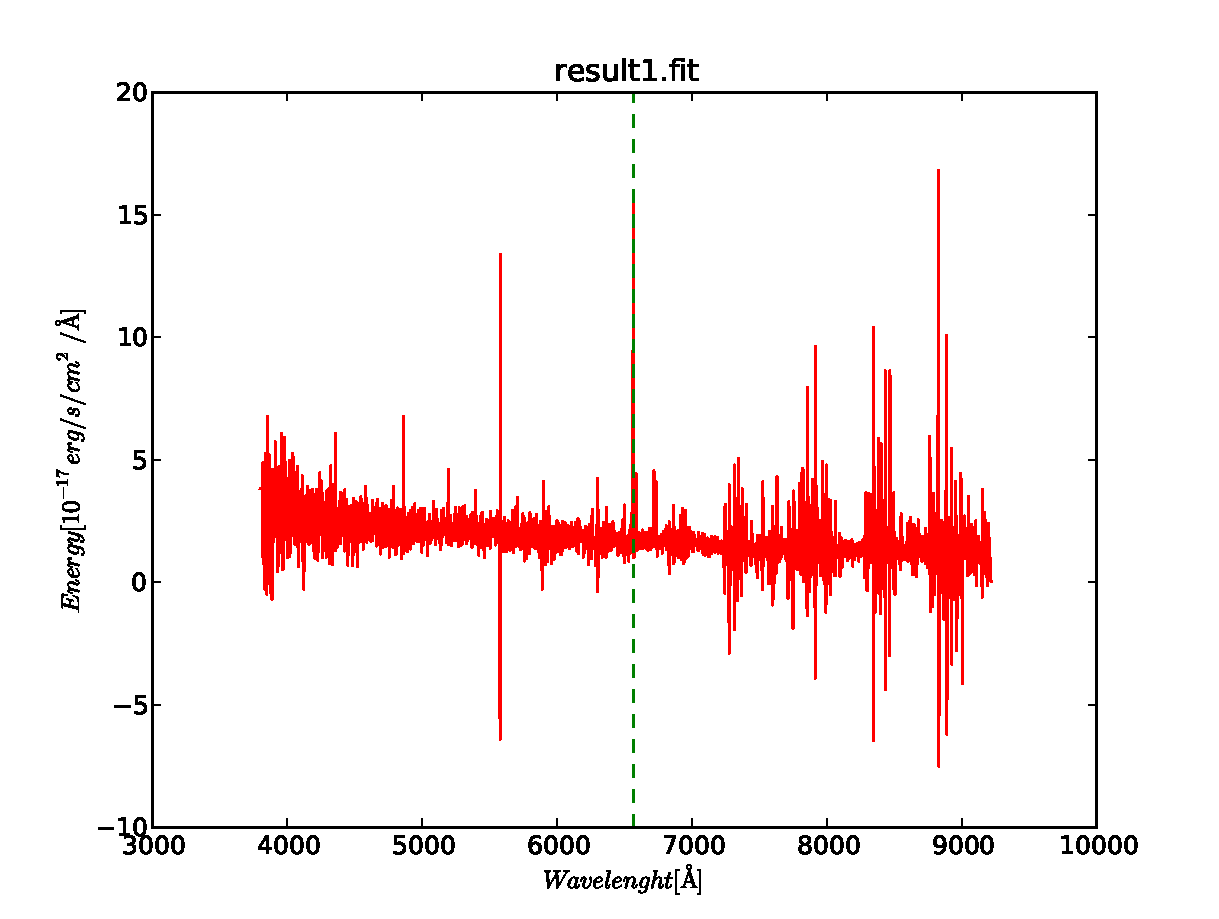
\includegraphics[scale =.6]{result1}
        \else
        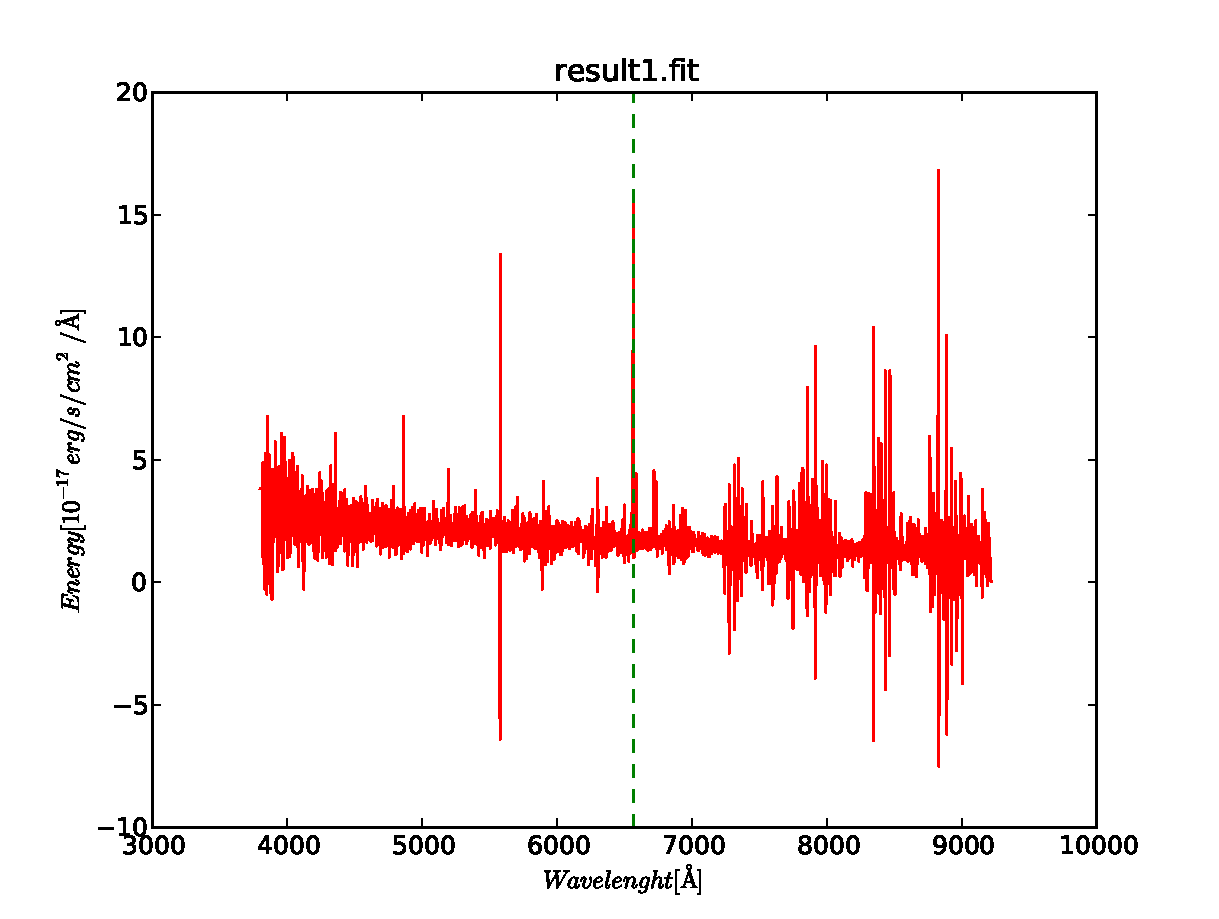
\includegraphics[bb = 92 86 545 742, height=6in]{result1}
        \fi
        \caption{Example 1: SDSS J035747.16-063850.7 }
        
        \label{FigResult1}
      \end{center}
    \end{figure}

   \begin{figure}[!htbp]
      \begin{center}
        \leavevmode
        \ifpdf
        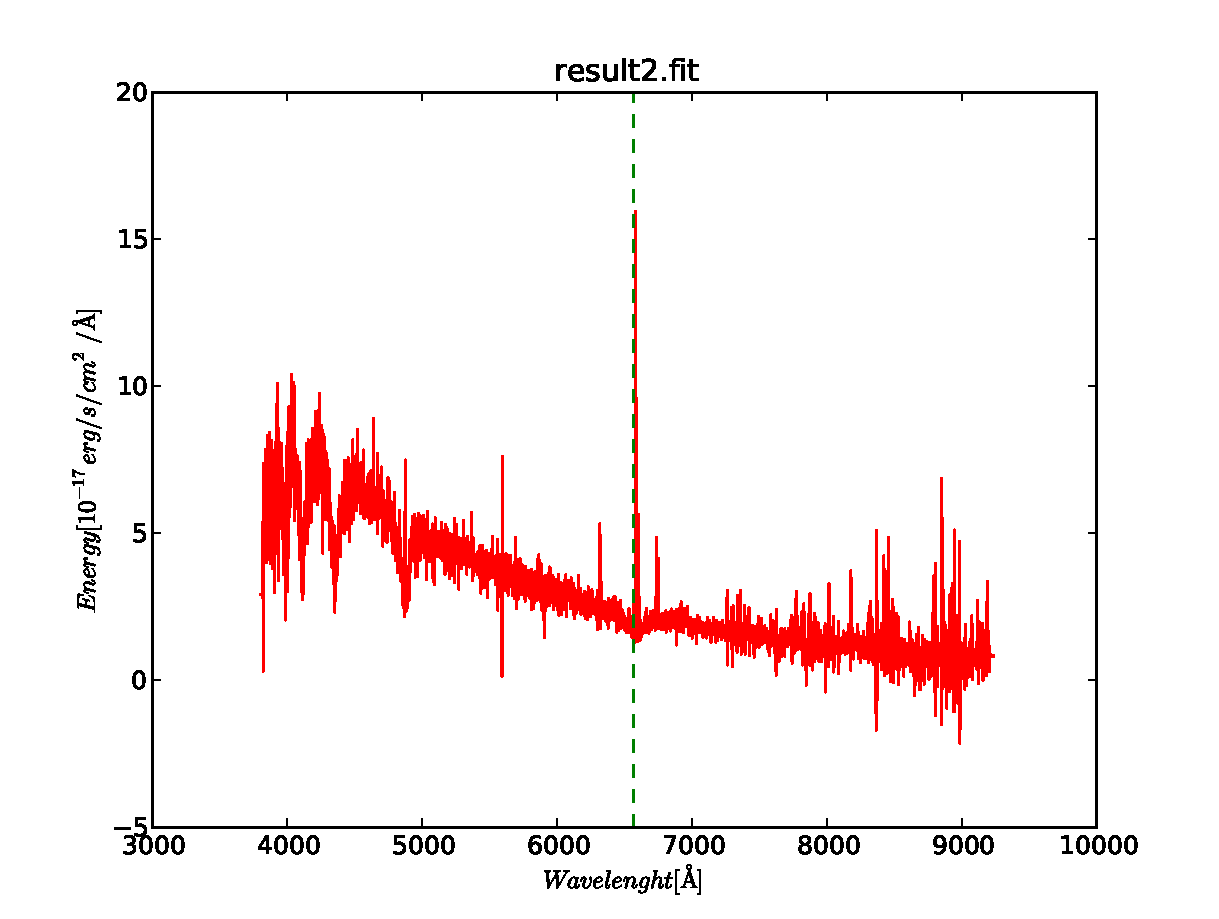
\includegraphics[scale =.6]{result2}
        \else
        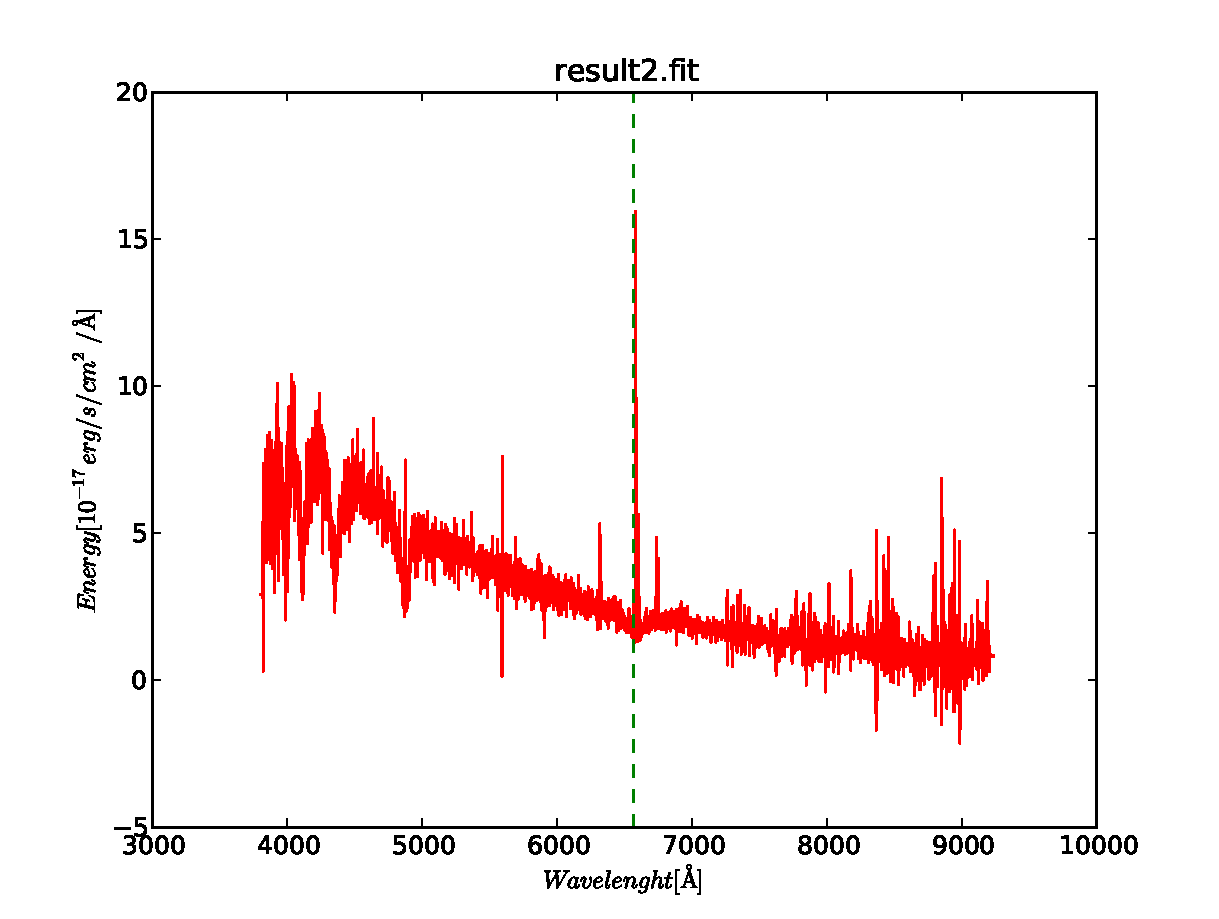
\includegraphics[bb = 92 86 545 742, height=6in]{result2}
        \fi
        \caption{Example 2: SDSS J094325.89+520128.6}
        \label{FigResult2}
      \end{center}
    \end{figure}

   \begin{figure}[!htbp]
      \begin{center}
        \leavevmode
        \ifpdf
        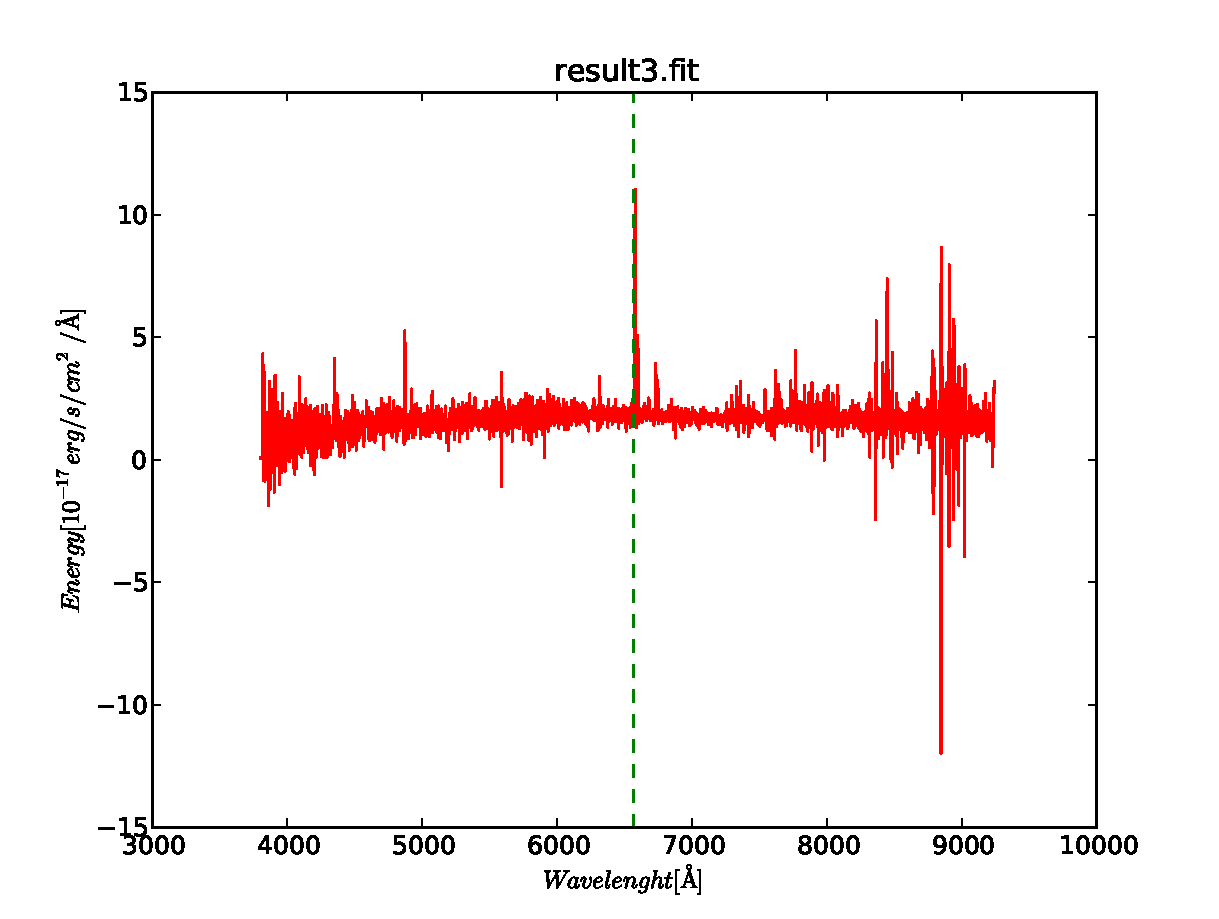
\includegraphics[scale =.6]{result3}
        \else
        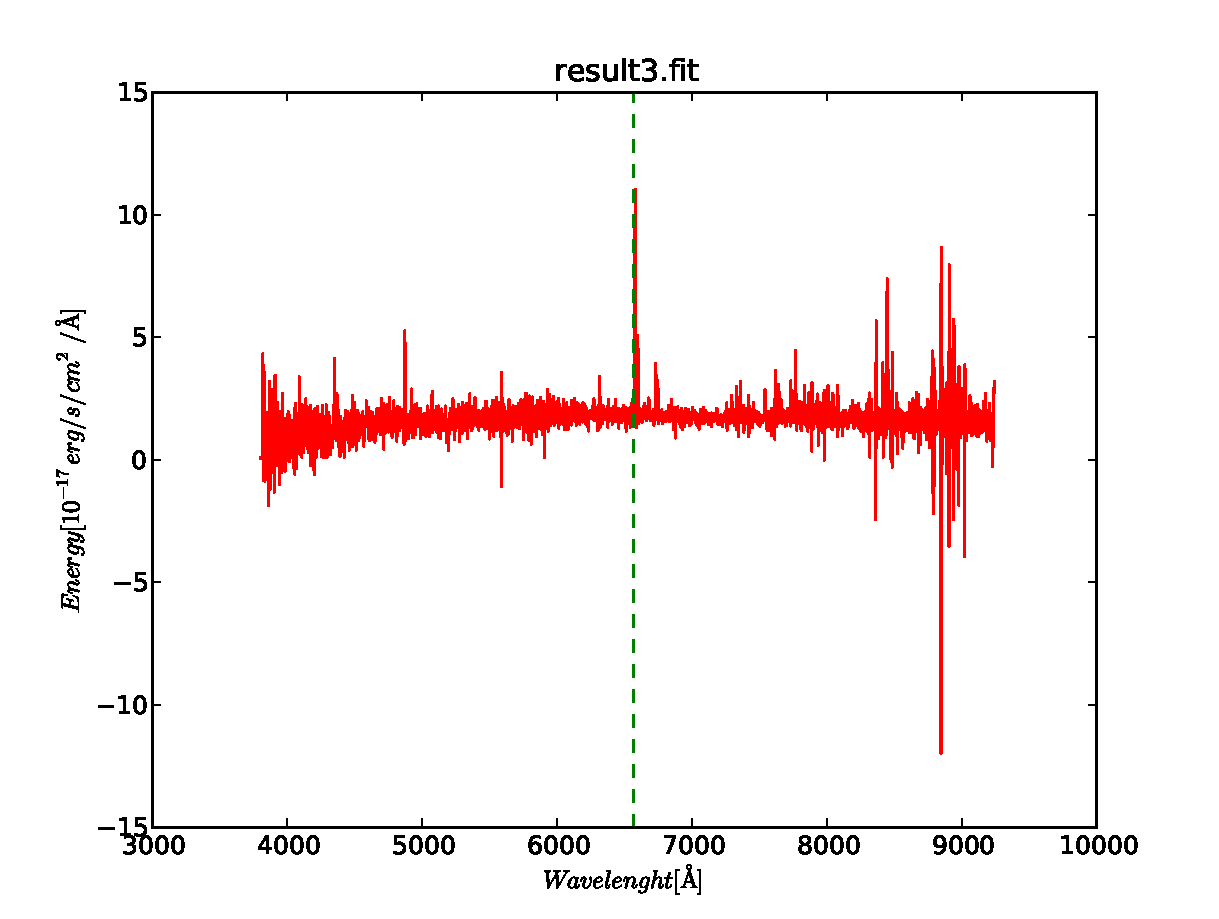
\includegraphics[bb = 92 86 545 742, height=6in]{result3}
        \fi
        \caption{Example 3: SDSS J120729.12+003659.8}
        \label{FigResult3}
      \end{center}
    \end{figure}

   \begin{figure}[!htbp]
      \begin{center}
        \leavevmode
        \ifpdf
        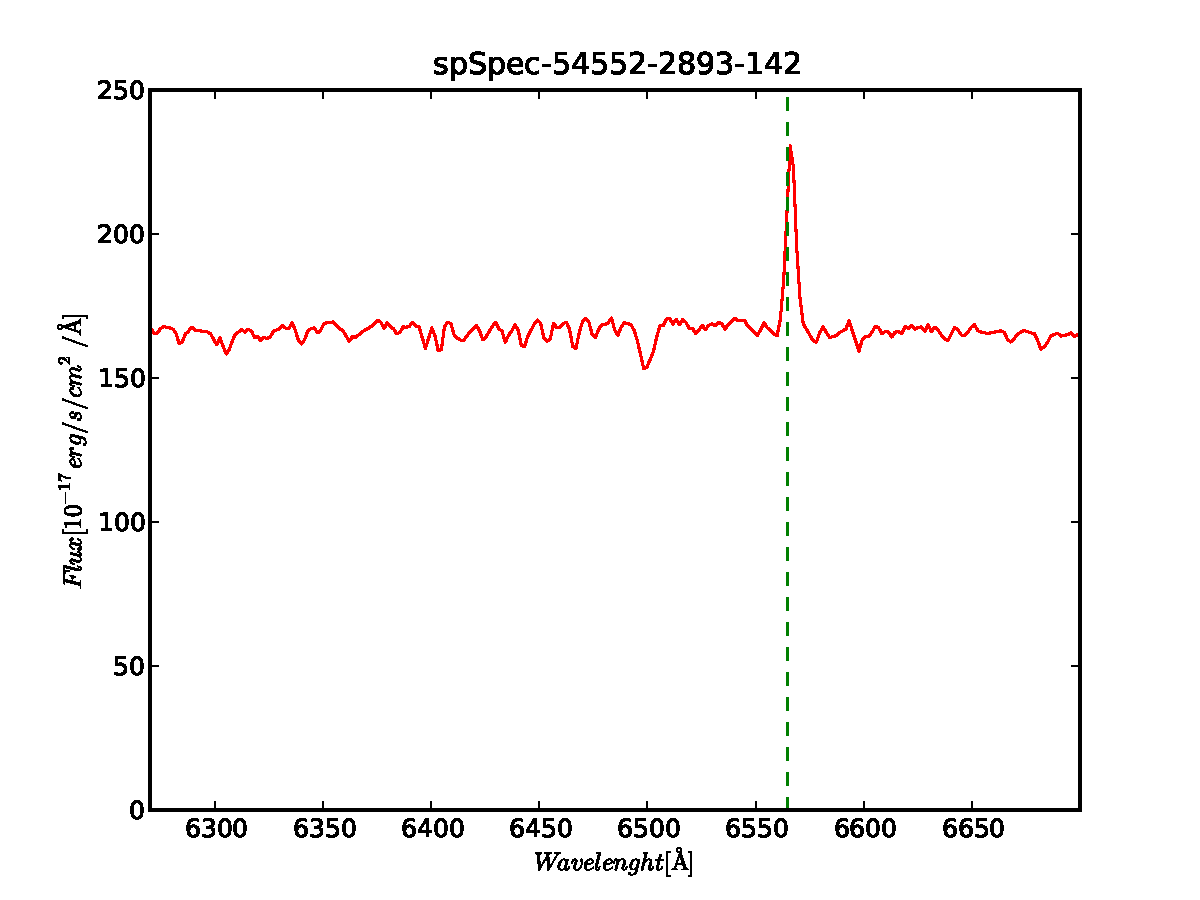
\includegraphics[scale =.6]{result4}
        \else
        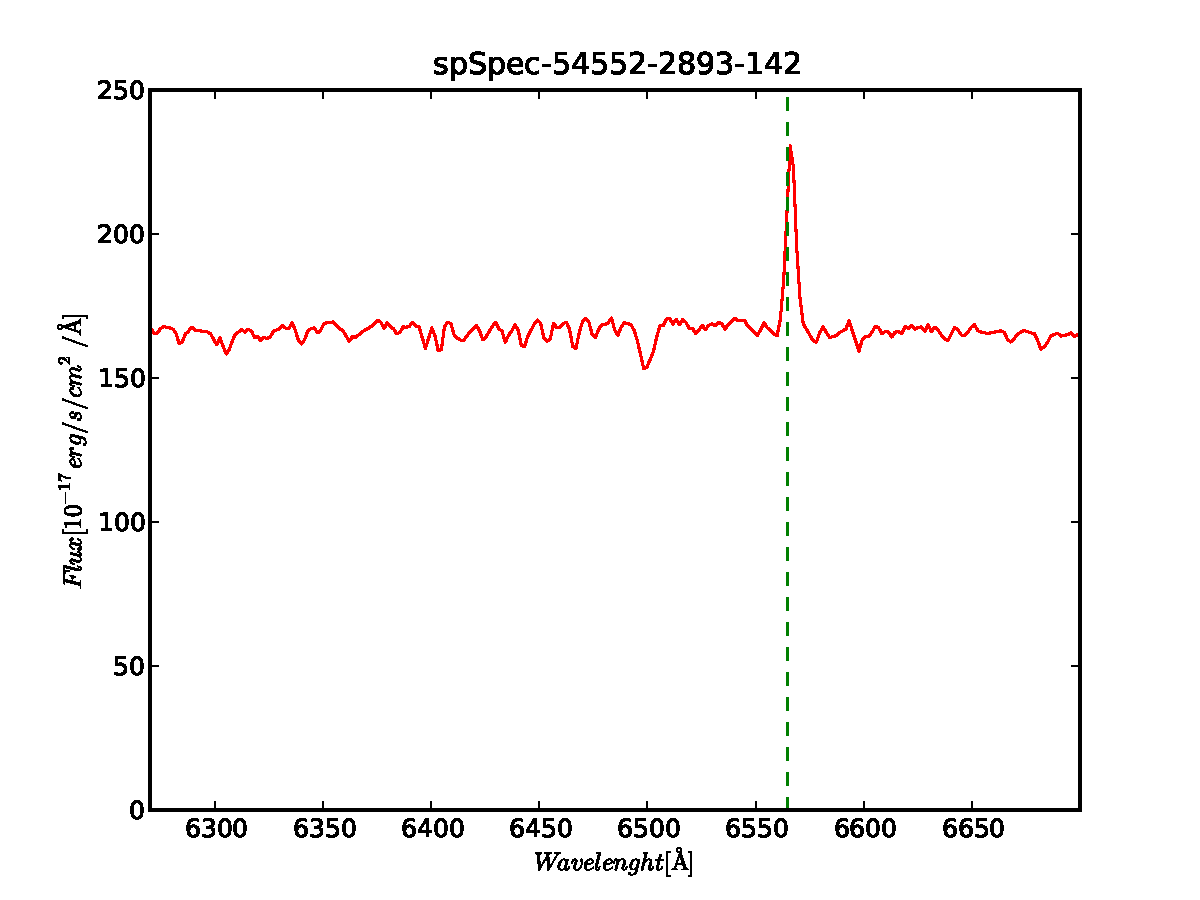
\includegraphics[bb = 92 86 545 742, height=6in]{result4}
        \fi
        \caption{Example 4: SDSS J120908.18+194035.8 }
        \label{FigResult4}
      \end{center}
    \end{figure}
%\clearpage

% Samples of Be Stars           
 
    For comparison there are spectra of known Be stars given in
    figures \ref{FigBe1},\ref{FigBe2},\ref{FigBe3} and
    \ref{FigBe4}. It is clear that the profile of the H$\alpha$ line
    is complex and just one parameter cannot possibly express it's
    characteristics. More advanced description such as wavelet
    coefficients or theoretical models of the line is needed if we
    want to create reliable process for identifying Be stars.

   \begin{figure}[!htbp]
      \begin{center}
        \leavevmode
        \ifpdf
        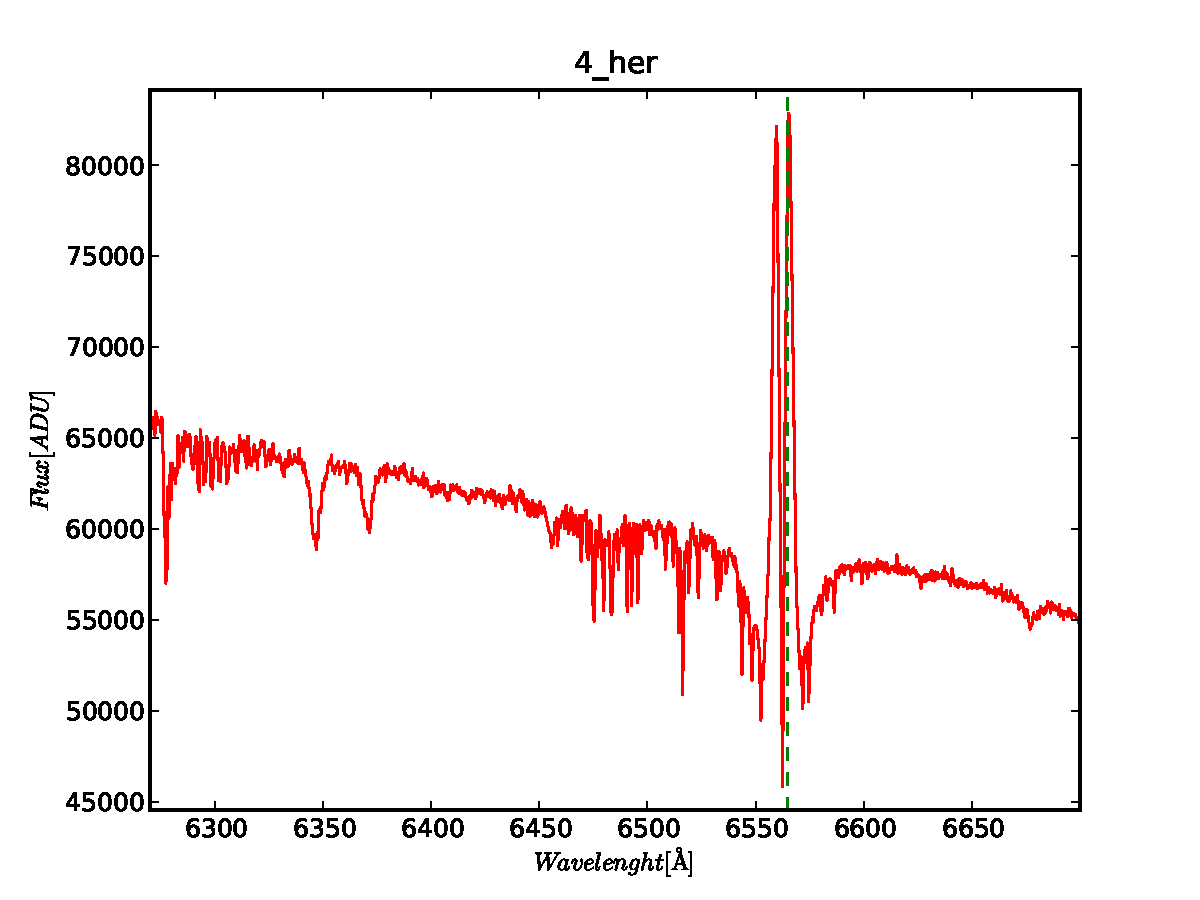
\includegraphics[scale =.6]{4_her}
        \else
        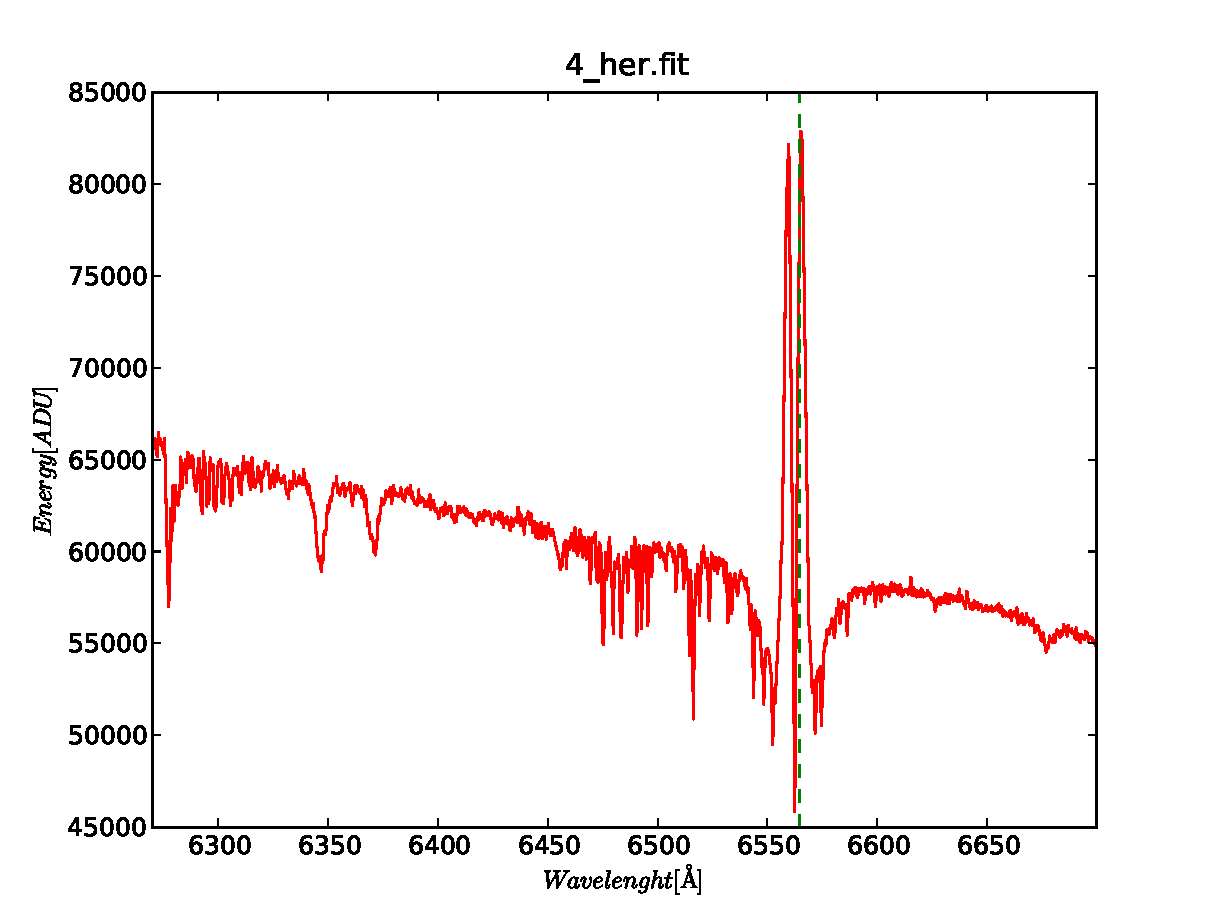
\includegraphics[bb = 92 86 545 742, height=6in]{be1_4_her}
        \fi
        \caption{Spectrum of 4 Her. Be star}
        \label{FigBe1}
      \end{center}
    \end{figure}

   \begin{figure}[!htbp]
      \begin{center}
        \leavevmode
        \ifpdf
        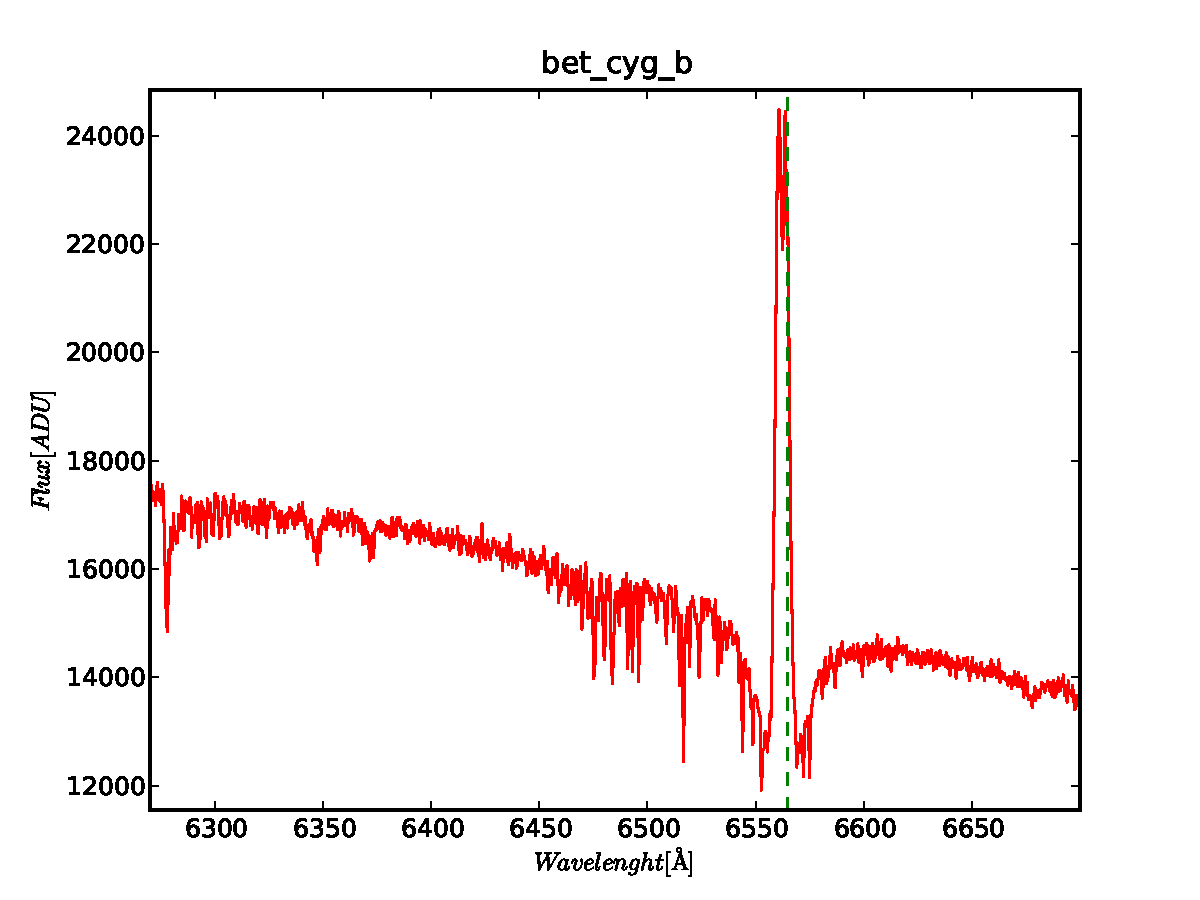
\includegraphics[scale =.6]{bet_cyg_b}
        \else
        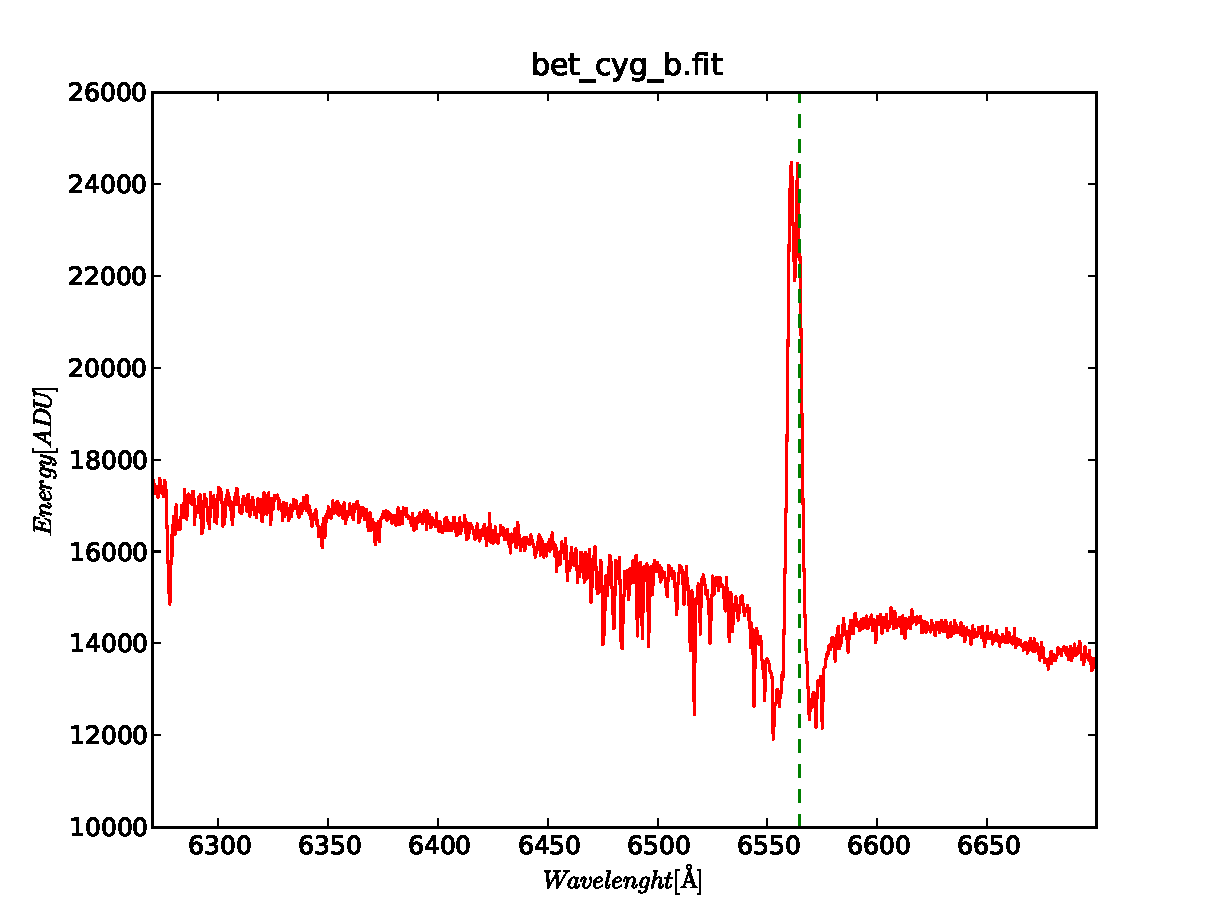
\includegraphics[bb = 92 86 545 742, height=6in]{be4_bet_cyg_b}
        \fi
        \caption{Spectrum of HR 7418 (Albireo B). A fast-rotating Be
          star, with an equatorial rotational velocity of at least 250
          kilometers per second. Its surface temperature has been
          spectroscopically estimated to be about 13.200 K }
        \label{FigBe2}
      \end{center}
    \end{figure}

   \begin{figure}[!htbp]
      \begin{center}
        \leavevmode
        \ifpdf
        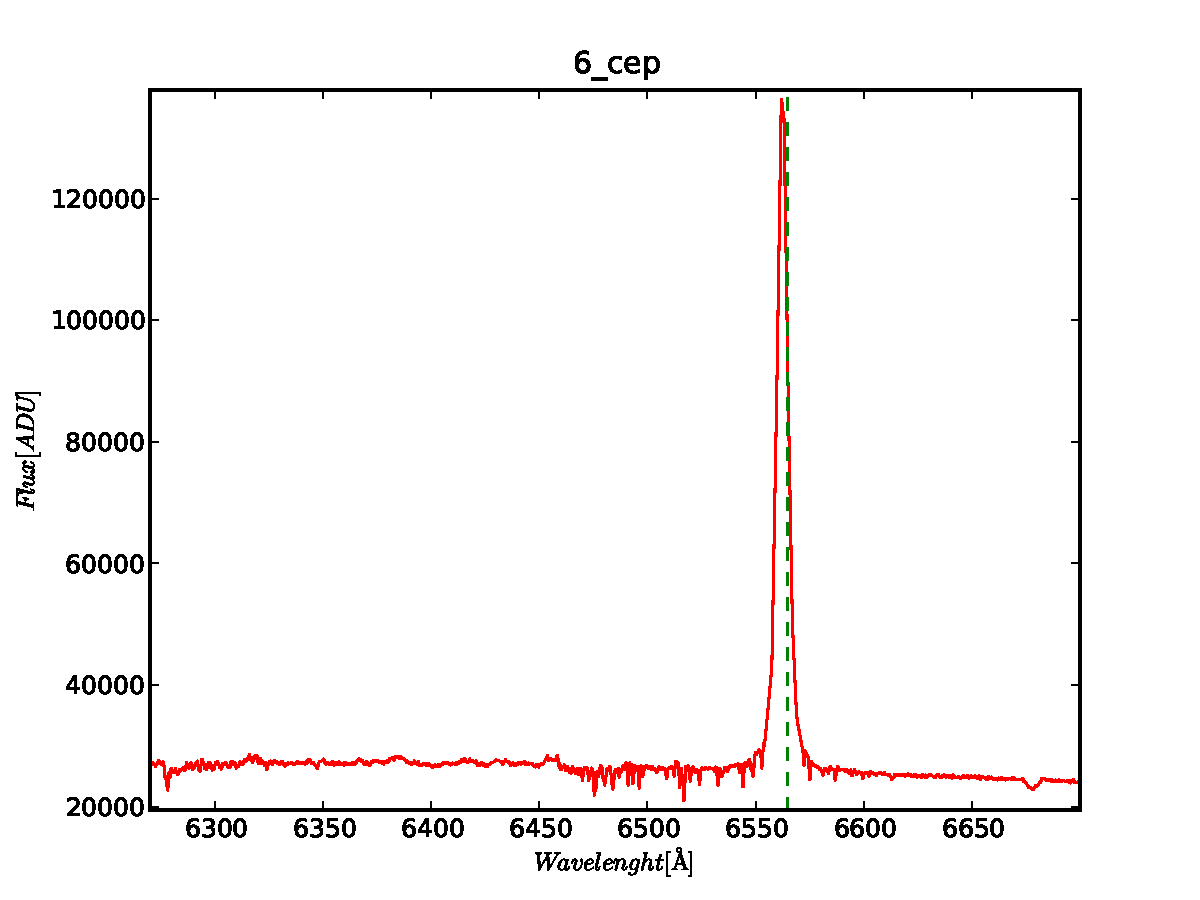
\includegraphics[scale =.6]{6_cep}
        \else
        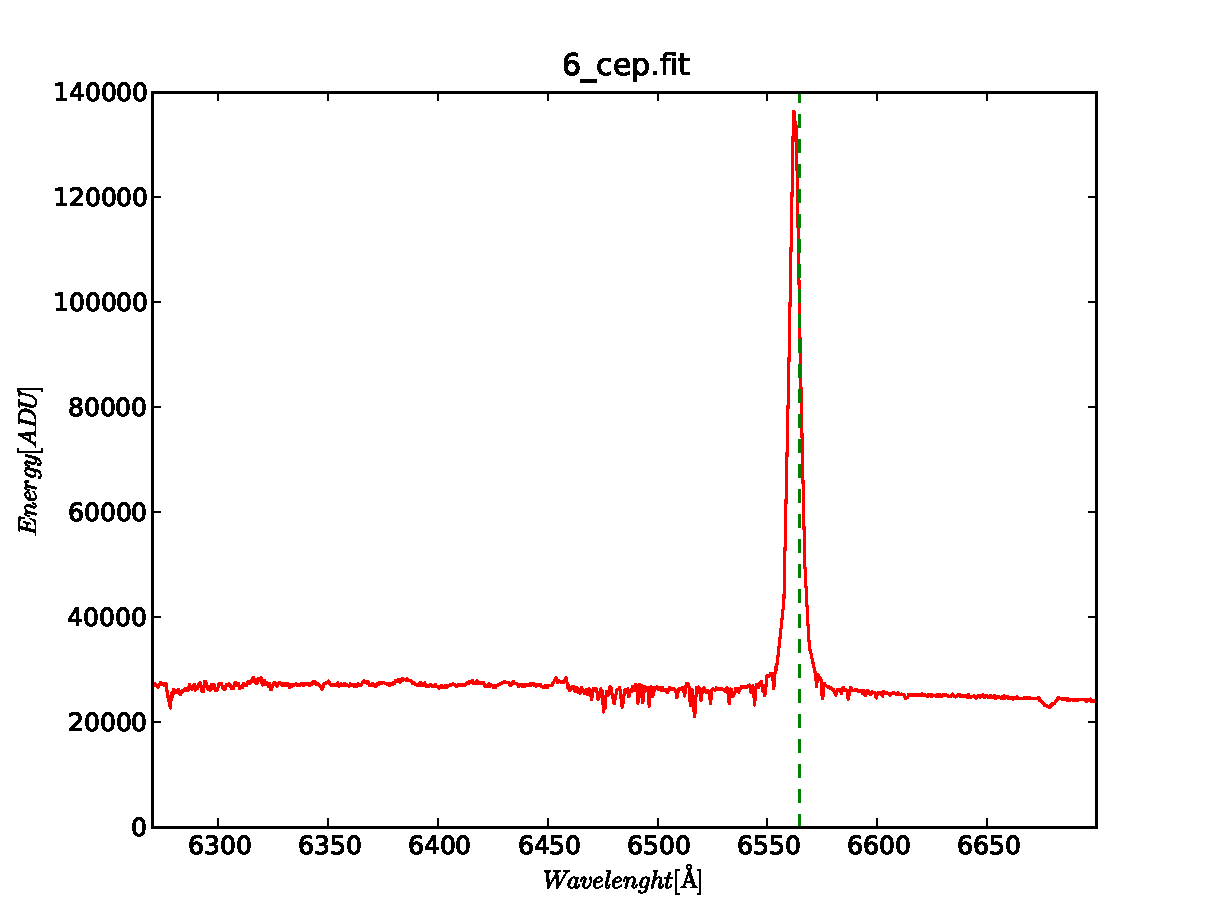
\includegraphics[bb = 92 86 545 742, height=6in]{be3_6_cep}
        \fi
        \caption{Spectrum of 6 Cep. Be star}
        \label{FigBe3}
      \end{center}
    \end{figure}

  \begin{figure}[!htbp]
      \begin{center} 
        \leavevmode
        \ifpdf
        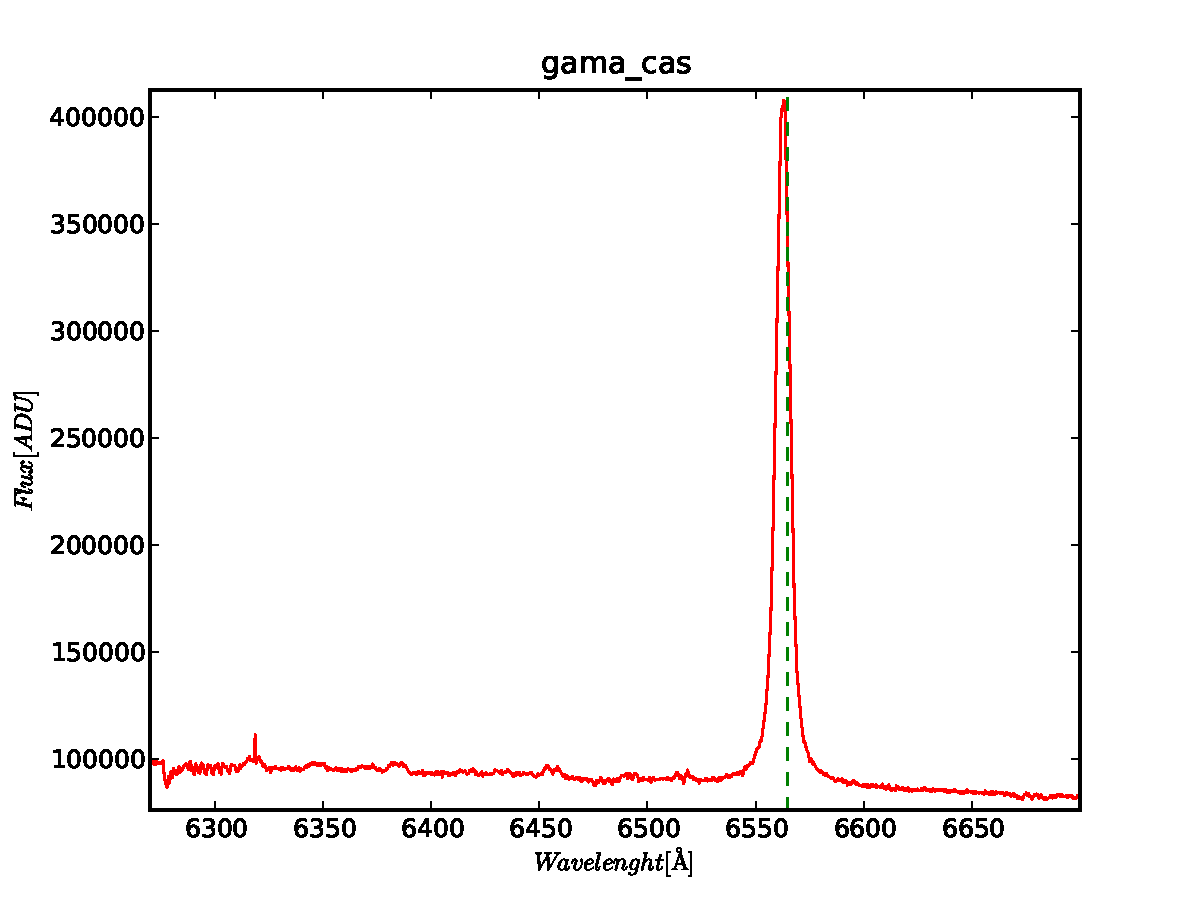
\includegraphics[scale =.6]{gama_cas}
        \else
        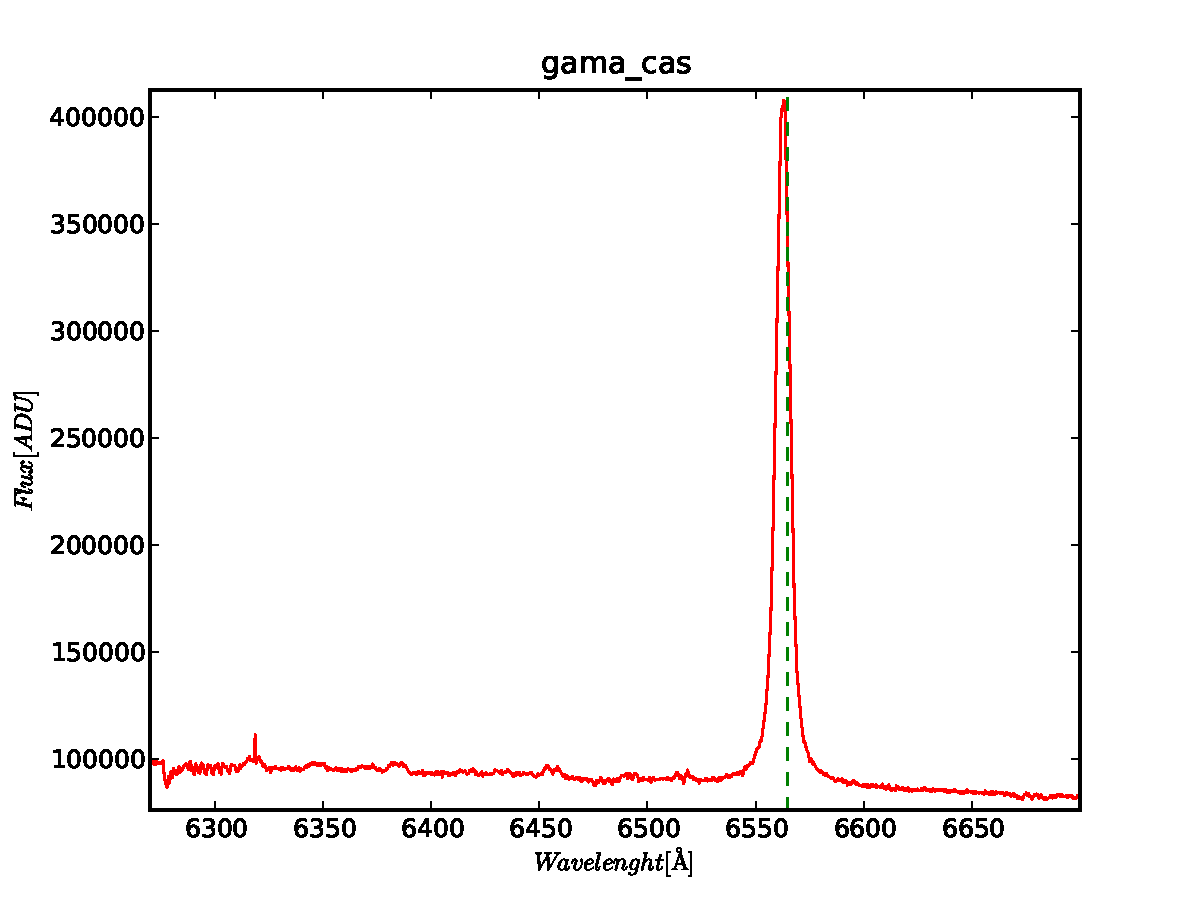
\includegraphics[bb = 92 86 545 742, height=6in]{gama_cas}
        \fi     
        \caption{Spectrum of Gamma Cas. Be Star}
        \label{FigBe4}
      \end{center}
    \end{figure}



%\clearpage

\subsection{Experiment}

One could be interested what would happen if we had chosen different
parameters, used other algorithm, different training set etc. These
are perfectly valid questions and it is actually the purpose and
essence of data mining and computers in general: to perform similar
tasks over and over again. With some automation in mind such
experiments are easy to do. Here is one of the test I have performed.

Natural idea one could have is using just a height of emission line
and write a program to check the spectra for condition \textrm{if
  emission $>$ threshold}. Then we do not need "expensive" data mining
algorithms to get some interesting results\footnote{This was actually
  done in the early stage of this project.}. Lets try to use
classification using just the height of the emission line (parameter
alpha). Here is consequent tree:


\begin{lstlisting}
  J48 pruned tree
------------------
alpha <= -0.464633
|   alpha <= -0.676474: be (45.0/18.0)
|   alpha > -0.676474: o (46.0/5.0)
alpha > -0.464633: be (92.0/16.0)
\end{lstlisting}

We can see that it is not so straightforward. In the training set
there are some Be stars with extreme height in the negative direction
(the spectrum obtained out of Be phase shows H$\alpha$ in
absorption). We have some statistics from classifier. In this example
the effectiveness was $77.6$\%. Also there is a confusion matrix,
which indicates how the classifier will fail to perform in individual
cases. Here it shows that it is almost exact when the object is Be
star but it confuses other types of stars with Be stars.

\begin{lstlisting}
  === Confusion Matrix ===
 Be     O   <-- classified as
 102    6 |   Be
  35   40 |   Others
\end{lstlisting}


This experiment proves that using data mining has a sense even in
apparently simple cases and can provide non-trivial insight on data
examined.


% Confusion Matrix indicates that the classifier is much better in
% predicting Be stars (102/6 correct assignments) then in predicting
% results in the \textrm{others} group where there are just 40/35 right
% assignments.




